\documentclass[12pt]{report}

\usepackage{graphics}
\usepackage{epsfig}
\usepackage{times}
\usepackage{amsmath}
\usepackage{booktabs}
\usepackage{subcaption}
\usepackage{wrapfig}

% Keyword Packages
% \usepackage{graphicx}
% \usepackage{subfigure}
\usepackage{algorithmic}
\usepackage{amssymb}
\usepackage{url}
\usepackage{algorithm}
\usepackage{epstopdf}
\usepackage{cite}
\usepackage{color}
\usepackage{ifthen}
\usepackage{newclude}
\usepackage[T1]{fontenc}
% \usepackage[latin2]{inputenc}
\usepackage{balance}

% Footprints packages
% \usepackage{epstopdf}
\usepackage{multirow}


\usepackage{hyperref}

% <http://psl.cs.columbia.edu/phdczar/proposal.html>:
%
% The standard departmental thesis proposal format is the following:
%        30 pages
%        12 point type
%        1 inch margins all around = 6.5   inch column
%        (Total:  30 * 6.5   = 195 page-inches)
%
% For letter-size paper: 8.5 in x 11 in
% Latex Origin is 1''/1'', so measurements are relative to this.

\topmargin      0.0in
\headheight     0.0in
\headsep        0.0in
\oddsidemargin  0.0in
\evensidemargin 0.0in
\textheight     9.0in
\textwidth      6.5in

% \title{{\bf Doctoral Thesis Proposal} \\
% \it Thesis proposal}
\title{{\bf Big Location Data: \\ Balancing Profits, Promise, and Perils} \\
\it Thesis Proposal}
\author{ {\bf Chris Riederer}  \\
Department of Computer Science \\
Columbia University\\
{\small mani@cs.columbia.edu}
}
\date{\today}

%%%%%%%%%%%%%%%%%%%%%%%%%%%%%%%%%%%%%%%%%%%%%%%%%%%%%%%%%%%%%%%%%%%%%%%%%%%%%%%
%%%%%%%%%%%%%%%%%%%%%%%%%%%%%%%%%%%%%%%%%%%%%%%%%%%%%%%%%%%%%%%%%%%%%%%%%%%%%%%
%%%%% COMMANDS
\newcommand{\chap}[1]{Chapter~\ref{#1}}
\newcommand{\fig}[1]{Figure~\ref{#1}}
\newcommand{\figwidth}{\textwidth}
\newcommand{\halfwidth}{0.5\figwidth}

\newcommand{\eg}{{\it e.g.}}
\newcommand{\ie}{{\it i.e.}}
\newcommand{\etc}{{\it etc.}}

%%%%%%%%%%%%%%%%%%%%%%%%%%%%%%%%%%%%%%%%%%%%%%%%%%
%% Stuff for "Keyword-Based Location Disclosure"



% Mathematical LaTeX formatting shortcuts
\newcommand{\midwor}[1]{\;\textnormal{ #1 }\;} % text in math mode
\newcommand{\ds}{\displaystyle} % shorcut to toggle display
	% All formula should punctuation as they are part of the text.
\newcommand{\vf}{\,,\,} % a comma with space
\newcommand{\ff}{\,.} % a dot 
	% The following command allows to write quickly sets { }   
\newcommand{\lset}{\left\{\left.\;}
\newcommand{\midset}{\;\right|\;\left.}
\newcommand{\dimset}{\right.\;\left|\;}
\newcommand{\rset}{\;\right.\right\}}
\newcommand{\jset}{\right.\right.\\ & \left.\left.}

% Number sets and usual operations
\newcommand{\Real}{\mathbb{R}} % real numbers
\newcommand{\RelInt}{\mathbb{Z}} % relative integer numbers
\newcommand{\NatInt}{\mathbb{N}} % natural integer numbers
\newcommand{\Compl}{\mathbb{C}} % complex numbers
\newcommand{\valent}[1]{\left\lfloor #1 \right\rfloor} % integer value
\newcommand{\valentsup}[1]{\left\lceil #1 \right\rceil} % integer value + 1
\newcommand{\eps}{\varepsilon} % very small real number
\newcommand{\argmin}{\textrm{argmin}} %argument of the minimum
\newcommand{\pospar}[1]{\left( #1 \right)^+} % positive part

% Probability notation
\newcommand{\proba}{\mathbb{P}} % Probability
\newcommand{\probaof}[1]{\mathbb{P}\left.\left[#1\right.\right]} % Probability of an event
\newcommand{\cond}{\right|\left.} % Condition on an event 
\newcommand{\expec}[1]{\mathbb{E}\left[#1\right]} % Expectation 
\newcommand{\vari}[1]{\textrm{V}\left[#1\right]} % Variance 
\newcommand{\Lun}{\mathbb{L}^{1}} % Space of integrable function
\newcommand{\as}{\;\textrm{a.s.}\;}
\newcommand{\ind}[1]{\mathbb{I}_{\{#1\}}} % Indicator
\newcommand{\tribF}{\mathcal{F}} % sigma-algebra

% Constants
\newcommand{\cst}{\textrm{\texttt{cst}}}

% Advanced probability 
\newcommand{\comp}{\circ} % composition of function
\newcommand{\shi}{\theta} % ergodic shift
\newcommand{\lstoc}{\displaystyle \leq_{\textrm{st}}} % Stochastic Order
\newcommand{\Ppalmof}[1]{\mathbb{P}^{0}_{#1}}
\newcommand{\Pofpalmof}[2]{\mathbb{P}^{0}_{#1}\left[#2\right]}
\newcommand{\expPalm}[1]{\mathbb{E}^{0}[#1]} % Palm Expectation
\newcommand{\expPalmof}[2]{\mathbb{E}^{0}_{#1}[#2]} % Palm Expectation w.r.t. point process f 

% (max,+) algebra
\newcommand{\Rmax}{\mathbb{R}_{\max}}
\newcommand{\ninf}{\varepsilon}
\newcommand{\matninf}{\textrm{\Large{$\ninf$}}}
\newcommand{\zer}{e}
\newcommand{\veczer}{\textrm{\Large{e}}}
\newcommand{\bigmax}{\bigvee}
\newcommand{\matId}{{\mathbb{I}}}
%\newcommand{\norm}[1]{\| #1 \|}
\newcommand{\linf}[1]{\left|\left| #1 \right|\right|}

% Matrices
\newcommand{\matA}{\mathbb{A}}
\newcommand{\matB}{\mathbb{B}}
\newcommand{\matC}{\mathbb{C}}
\newcommand{\matP}{\mathbb{P}}
\newcommand{\matQ}{\mathbb{Q}}

% Used for set
\newcommand{\setI}{\mathcal{I}}
\newcommand{\setJ}{\mathcal{J}}
\newcommand{\setK}{\mathcal{K}}
\newcommand{\setL}{\mathcal{L}}

% Users and Buckets
\newcommand{\setU}{\mathcal{U}}
\newcommand{\setC}{\mathcal{C}}

\newcommand{\setA}{\mathcal{A}}
\newcommand{\setW}{\mathcal{W}}

% Used for set
\newcommand{\setN}{\mathcal{N}}
\newcommand{\setS}{\mathcal{S}}


\newenvironment{disarray}%
 {\everymath{\displaystyle\everymath{}}\array}%
 {\endarray}

 \newcommand{\pdi}[1]{\frac{\partial #1}{\partial x_i}}
 \newcommand{\pdj}[1]{\frac{\partial #1}{\partial x_j}}


\definecolor{myviolet}{rgb}{0.4,0.0,0.7}
\definecolor{heraldBlue}{rgb}{0.0,0.0,0.8}
\definecolor{heraldRed}{rgb}{0.8,0.0,0.0}
\definecolor{heraldGray}{rgb}{0.4,0.4,0.4}
\definecolor{heraldBlack}{rgb}{0.0,0.0,0.0} %removes comment color
\definecolor{heraldGreen}{rgb}{0.0,0.4,0.0} %removes comment color
\def\r#1{\textcolor{heraldBlue}{\em #1}}
\def\q#1{\textcolor{heraldRed}{\em #1}}
\def\d#1{\textcolor{heraldBlue}{#1}}
\def\R#1{\textcolor{heraldBlue}{#1}}
\def\D#1{\textcolor{heraldBlue}{#1}} 

\newcommand{\crnote}[1]{\textcolor{heraldBlue}{\small \bf [CR: #1]}}
\newcommand{\bknote}[1]{\textcolor{heraldRed}{\small \bf [BK: #1]}}
\newcommand{\venote}[1]{\textcolor{heraldGreen}{\small \bf [VE: #1]}}
\newcommand{\acnote}[1]{\textcolor{red}{\small \bf [AC: #1]}}
\newcommand{\changed}[1]{#1}

% Main set
\providecommand{\setL}{\mathcal{P}}
\providecommand{\setK}{\mathcal{K}}
\providecommand{\setU}{\mathcal{U}}

% Relevance factor, Revenue
\providecommand{\matA}{{A}}
\providecommand{\Rev}{{R}}
\providecommand{\Revtot}{{U}}

% Signature
\providecommand{\setH}{\mathcal{H}}

\providecommand{\setvecS}{\textrm{\textbf{S}}}
\providecommand{\setS}{\mathcal{S}}

\newcommand{\Succ}{\textrm{Succ}}
\newcommand{\Prec}{\textrm{Prec}}

\newcommand{\cpc}{\textrm{\texttt{CPC}}}
\newcommand{\rev}{\textrm{R}}
\newcommand{\argmax}{\textrm{argmax}}
\newcommand{\purU}{\widehat{\setU}}

\providecommand{\setP}{\mathcal{P}}




\begin{document}
\pagestyle{plain}
\pagenumbering{roman}
\maketitle

\pagebreak
\begin{abstract}
The ``Big Data" era has a lot of potential.
Businesses hope that Big Data will make them more efficitient and profitable or enable entirely new products.
Governments hope to provide better for the needs of their citizens.
At the same time, these new collections of data can present societal risks, as we've now enabled mass surveillance, a loss of privacy, and algorithmic bias.

The rise of cheap and ubiquitous electronics, including but not limited to smartphones, has enabled the capture and use of human mobility data like never before.
As a subset of Big Data, location data can be a boon to both profit centers and scientific understanding, but comes with many risks attached.
The places we visit can reveal much about ourselves, whether proclivities towards particular type of food, or more private characteristics of race, religion, sexuality, or political affiliation.

In this thesis proposal, I describe recent work that attempts to balance the scientific and engineering promises of location data with the potential risks.
I will describe work I have completed relating location data to privacy, anonymity, economics, and algorithmic bias.
I propose future research to be completed in the form of a thesis, advancing knowledge of location-based demographics and algorithmic bias.

\end{abstract}

\pagebreak
\tableofcontents
\pagebreak

\cleardoublepage
\pagenumbering{arabic}

% \section{Introduction}
\chapter{Introduction}
\label{ch:intro}
% Ermergerd big data
The era of Big Data has the potential to transform all aspects of society, from business operations to individual leisure time, from medicine to elections.
As the cost of computation and data storage has fallen, and as more human behavior has moved to easily-recorded digital mediums, both public and private institutions have captured and stored more and more information.
``Data is the new oil", analysts have proclaimed, as businesses seek to become more efficient or create innovative digital products. % TODO: cite
``Data will power the cities of tomorrow" governments have proclaimed, releasing their troves of data to the world.

% Shift: what are the problems
The excitement of the potential gains has been tempered by many potential concerns.
% Anonymity: NSA
With the desire for public agencies that could more accurately prioritize safety concerns has come massive surveillance, both by companies and governments, raising concerns of \textbf{anonymity}. % TODO: cite
% Economics: price discrimination
With the belief that Big Data would lower costs and benefit consumers has come evidence of large-scale price discrimination~\cite{wsj, Anonymous:2012wi}, with its impacts possibly most felt by already economically vulnerable populations, raising concerns of \textbf{economics}.
% Algorithmic bias: bail-setting
And with the hopes of making government more fair and efficient have come allegations that seemingly impartial algorithms actually encode unfair racial biases~\cite{propublica:bias}, raising concerns of \textbf{algorithmic bias}.
We must carefully consider how to obtain the benefits of the Big Data Age without paying too high a price.

% Location data
% Although Big Data encompasses the massive colletion of information from all areas of human activity, of particular interest and concern is data generated by the everyday activity of human beings, as this 
One particularly interesting and sensitive subset of Big Data is information relating to the real world movements of individuals: ``location data".
As this data is tied to actual physical movements, it is of enormous interests to businesses and governments.
When people move, they are expending energy and money to do so, as opposed to the many relatively low-cost digital behaviors captured online.
Thus, location data provides a valuable input for many problems, as evidenced by academic proof-of-concepts and by the many businesses and services surrounding it's capture, such as Google Location Services, Foursquare\footnote{\url{foursquare.com}}, Placed\footnote{\url{placed.com/}}, and many more.

% Problem: how to use location data safely?
% TODO: explain a bit more about what this case was about?
Along with its valuable signal again comes concerns of safety and privacy.
In the United States v. Jones decision, in which the Supreme Court wrestled with the legality of law-enforcement placing a GPS tracker on a car without a warrant, Justice Sotomayor wrote 
``disclosed in [GPS] data ... [are] trips the indisputably private nature of which takes little imagination to conjure: trips to the psychiatrist, the plastic surgeon, the abortion clinic, the AIDS treatment center, the strip club, the criminal defense attorney, the by-the-hour motel, the union meeting, the mosque, synagogue or church, the gay bar and on and on"~\cite{jones2012us}.
Clearly, if location data is to be used by analysts, it must be done so in a way that is extremely careful and respectful of user preferences.
% TODO: add another sentence

In this thesis proposal, I examine work that attempts to reconcile the benefits of data-mining location data with three key areas of concern: anonymity, economics, and algorithmic bias.
I will begin with a background section which introduces the core concepts found in this proposal, continue with several chapters relating to the afore-mentioned areas of concern, and conclude with a final discussion of next steps in making big location data safe and fair to use.

\section{Anonymity}
% Linking Users Across Domains with Location Data
% FindYou
\chap{sec:anon} examines the possibility of anonymizing location data. %TODO: edit
Prior work has shown that users are highly unique in their location patterns, leaving them vulnerable to de-anonymization (see~\ref{sec:privacy}).
Here we take this a step further, showing not only that this vulnerability exists, but that users indeed can be linked to other datasets.
Additionally, we provide a tool to users that aggregates and displays their location data along with the potential inferences made from it.

\section{Economics}
I focus on location data, privacy, and economics in \chap{sec:econ}.
We begin with work that seeks to understand user attitudes to their privacy and the economic value of their information.
Specifically, it examines an alternative to the current practice of firms offering free services in exchange for full control over user data.
The alternative model is one in which users control their data and make decisions about when to sell access to their info, and to whom.


\section{Algorithmic Bias}
% I Don’t Have a Photograph But You Can Have My Footprints
% Under submission work on demographic labeling
% Current work on bias!
Finally, I analyze the interaction between location data and algorithmic bias in \chap{chap:bias}.
We gather a dataset of locations attached to demographic information from a popular image-sharing mobile application.
This data allows us to study the differences in human mobility across different groups, and moreover, to show that demographics can be inferred using only location data.
This raises questions about the sensitivity of location data, and about the potential for bias in systems that make decisions based on location data.
We examine other methodologies for inferring demographics from social network data and discuss debiasing of algorithms.
Furthermore, I demonstrate a personal auditing tool for users to understand their location data and the inferences potentially made about them.

\section{De-biasing Location Based Advertising}
\chap{chap:proposal} links my previous works together in my proposal for future work.
I hope to discover the conditions under which adveritisers may safely use location data to decide when to show ads without unfairly benefiting one demographic group at the cost of another.
% This work will require an understanding of the 
Advertisers (and other users of algorithms) often wish to target users based on certain traits (e.g. interest in a product).
These users may be clustered geographically, for example, only users in New York will be interested in purchasing a subway pass for that city.
While wishing to target, advertisers may also wish to \emph{not} exclude certain demographics due to issues of fairness (and potential bad publicity).
Our New York City subway pass advertiser might not wish to offer more deals to the wealthy at the expense of the poor, for example.
By using a large dataset of location data tagged with user generated text and demographic information, I will be able to determine the cost of altering a location-based advertising algorithm to insure that ads are shown to a representative population.
A key metric will be demographic mobility, looking at how skewed from the overall distribution the make up of visits by certain demoagrphics are in a location.
In locations where the difference in demographic mobility is small, advertisers can tweak their algorithms to show ads equally across demographics with minimal cost, fair to both individuals and overall groups.
In other cases where the difference is large, the costs will likely be higher.
I offer more detailed description of this planned work in \chap{chap:proposal}.

% I discuss my plans to analyze real world algorithmic bias in a location-based advertising setting along with my current progress.

% \chap{sec:proposal-ii}

% I conclude with a plan for completing this work in \chap{sec:plan}.


  \section{Background}
  \label{sec:background}
  % \subsection{Location Data}
\textbf{What is location data?}
Most generally, location data is information relating people to places.
Typically, this relation is the fact that a person was at a place.
Adding time into the figure, the relation could be that a person was at a place at a particular time.
However, location data could also include relations about the importance of a place in someones life, such as them living in a location, working at a location, or having spent a quantity of time in a location.
Though location data does not need to be associated with user IDs, in this work we will consider that there is always attached some sort of user ID that uniquely identifies the user in the dataset, possibly de-personalized.

Location data can be described in two main ways: \textbf{geographically} or \textbf{semantically}.
\emph{Geographic} data can be described by a latitude-longitude data on the globe.
\emph{Semantic} location data refers to an identifier used within that dataset.
This could have some information available to a common user, e.g. ``New York City", or it could simply be an identifier, e.g. 7.
Note that often these two may be combined or used together.
A location such as ``CEPSR Office 618, Columbia University" (the author's office) indicates a very small, non-ambiguous location that can easily be mapped to geographic coordinates.
Semantic location data can sometimes present a privacy problem, as an association with a place could indicate sensitive attributes, such as someone's religion, political affiliation, health, or sexuality.
In this work, I will typically assume location data is also tagged with temporal data, and I will use the terms location data and spatiotemporal data interchangeably.

To put this more formally, we can define a single data point $p$ of location data to be:
\[ p = \langle u, l \rangle \]
or, including time:
\[ p = \langle u, l, t \rangle \]
where $u$ uniquely identifies a user, $l$ uniquely identifies a location, and $t$ specifies a time.
Note that $l$ could be a latitude-longitude pair in the geographic case or an ID in the semantic case.

\textbf{How is location data collected?}
Location data can be captured passively or actively.
\textbf{Actively captured} location data is only recorded when the user takes some action.
Note that this action does not need to inherently be ``about" location data, for example, a user making a call from a cell phone or swiping a credit card is typically not consciously thinking about their location data. 
A record of their location is created as a by-product of their use of that technology.
\textbf{Passively captured} is meant in a stronger way-- the user's location is captured without the user making any kind of action.
This can occur through tracking apps.
An example is MapMyRun\footnote{\url{http://www.mapmyrun.com/}}, an app where users record their routes while running, in order to track distance and progress in meeting exercise goals.
Although the user took an action to start recording their location, the location is recorded in the background with no user action from then on, and hence we call it ``passive".
Another example is Google's location history.
Google records location data in the background of a users Android phone every few minutes.
A map of everywhere a user (with an Android phone with location history turned on) is available at \footnote{\url{https://www.google.co.in/maps/timeline}}.

% \textbf{What is location used for?}
% TODO



% \subsection{Privacy}
% \label{ssec:privacy}
% Privacy has been an important concept, brought to the forefront of public debate as surveillance of users has grown, both by governments and private companies.

% ADD MORE STUFF

% In this work, we will focus on two technical conceptions of privacy, \emph{k-anonymity} and \emph{differential privacy}.

% \textbf{k-anonymity} 

% \textbf{Differential privacy}


% \subsection{Bias}

% \subsection{Online Advertising}



\chapter{Location Data and Anonymity}
% \section{Location Data and Anonymity}
\label{sec:anon}
Linking Users Across Domains with Location Data


and

FindYou



\chapter{Location Data, Privacy, and Economics}
% \section{Location Data, Privacy, and Economics}
\label{sec:econ}
% Introduction

% The primary goal of big data is to guide decision making.
The online attention economy is based primarily on advertising.
Some of the most powerful and far-reaching online services, such as Google and Facebook, operate mostly with free services.
The income of a firm roughly translates to (number of impressions) x (dollars per impression).
Firms are not necessarily paid on an impression basis, as other models like paying per click or per sale or other action are quite common, but it is reasonable to think of clicks or sales as some function or subset of impressions.
Fundamentally, much of the dollars in profits given to online firms are based on how many people come to their site and how well they can target advertisements to those individuals.
This gives firms an incentive to gather as much information about their users as possible so that they can better target ads to them.

% sec:background
% This can of course present a privacy issue.
This framework presents a challenge to privacy.
User information is collected and gathered in one centralized place.
There are multiple risks involved here: the firms themselves may use the information in ways the users disagree with, the firms may sell or be coerced to give their information to other firms or governments, or the firms may fall victim to cybersecurity attacks, leaking information to other sources.

As ways to counter this, schemes have been proposed to encrypt user behavior and information, denying all access to a firm.
However, this would deny firms the ability to make money, meaning no services would be provided for users and possibly a lower global utility be reached.
Thus, schemes that ignore this economy however are unlikely to be adopted.
Companies need to make money to function.
Currently, users seem happy to provide their data in exchange for free services.
A concern is that users do not have a good idea of their data and do not know how it is being used and to whom it is accessible.

Therefore it is important to gain an understanding of how users value their information, what they believe firms are doing with their data, and what users are comfortable with in terms of data use.
Building upon my previous work analyzing how users value their information~\cite{Carrascal} and proposing alternative data discolure methods~\cite{Riederer:2011ta}, in this section I propose a new method for representing user locations in a privacy sensitive manner that can still be effective for advertisers.


  \section{User Choice in Location Disclosure}
  % \section{Location Data, Privacy, and Economics: \\User Choice in Location Disclosure}
  \label{sec:keyword}
  % \subsubsection{Challenges of Keyword-Based Location Disclosure}

% The rapid adoption of smart phones and tablets has led to innovative applications and services
% that exploit location information. Location information is increasingly used to
% drive advertising -- location-based targeting generates four times as much revenue per impression compared to ads 
% without location data\footnote{\url{http://bit.ly/vXWdsw}}. Even brick-and-mortar stores use location data, with retailers 
% using cell phones' WiFi signals to learn where customers spend time in their stores\footnote{\url{http://nyti.ms/15vLRva}}.

% There are many privacy concerns surrounding the use of this data.
% %Location information is more sensitive than other types of personally identifiable information (PII) not only because it can reveal private activities, but because knowledge of a person's physical presence creates the possibility of physical harm.
% For example, many applications access location information even when such information is not needed, and may share it 
% with multiple third parties, leading to privacy concerns~\cite{Enck:2010, WSJ:apple} and attracting 
% the attention of regulators~\cite{USC:location, jones2012us}.
% This work focuses on location information generated in real-time by users with mobile devices.

Many privacy concerns around location information are rooted in the mobile application ecosystem.
Most mobile services and applications are free and operate by collecting 
personal information (browsing activity, location, etc.) and monetizing this information 
through targeted ads~\cite{Leontiadis:2012}. 
% Because it affects their profits, companies that are a part of the mobile application ecosystem oppose any regulation that may restrict access to location data and claim that the ``cost'' of a privacy bill threatens the web's general economy and ultimately hurts customers. 
In fact, one may argue that users today exchange their data for services.
An ideal privacy solution therefore should provide adequate privacy protection to the user while simultaneously enabling service providers to collect and monetize data. 
Our objective is to lay the groundwork for a comprehensive and deployable solution to location privacy. 

In this section, I describe published work~\cite{Riederer:2013ila} that aims to reconcile the users' control over their location information with its commercial value.
This approach raises three challenges:
(1) The solution should be \emph{incrementally deployable}. 
It must easily integrate with current devices and practices while giving all parties an incentive to participate.
(2) The solution should be \emph{robust} against threats from its participants. 
Advertisers should not be able to access data without compensating users or access more than the users specify. 
Users should not be able to benefit from seeking unfair compensation.
(3) The solution should be \emph{easy to use}. 
The system should be easily understood by both users and advertisers.

Our solution is based on selective disclosure; users decide what location information they want to disclose.
At the heart of our solution is a \emph{keyword-based} method where keywords are associated with locations, and the decision to release locations is based on keywords. 
We observe that keywords are naturally associated with the elements that define this problem, but also offer a strong abstraction to handle location data.  
In order to drive the adoption of the solution, we propose providing economic compensation to the users for the location information they disclose. 
Application and web service providers bid to gain \emph{access} to users at these specific locations in real-time. 

\subsection{Overview}
Our requirements calls for a solution to share information about location monetized by ad-networks and 3rd party aggregators through \emph{selective disclosure}. For the user to retain control, our privacy solution should address \emph{how} the information is released, under \emph{which conditions} the information is released and to \emph{whom}, as seen in previous ones, e.g.~Koi~\cite{guha:koi}, 

% To meet our requirements, we create a solution based around \emph{selective disclosure}; users disclose location information that they are willing 
% to release.
% This information is monetized by ad-networks and third party aggregators by way of online ads. 
% The control remains with the user. 
% Any privacy solution based around selective disclosure 
% needs to
% address 
% \emph{how} the information is released, under \emph{which conditions} the information is released and to \emph{whom}.

To specify \emph{how} and \emph{under which conditions} location information is released, we choose to use keywords. 
While the information that is released is a latitude longitude pair (lat-long), the decision to disclose is based on associated keywords. 
Users who are comfortable disclosing location under certain circumstances~\cite{Kelley:2011} opt-in to reveal lat-long associated with keywords of their choices.
%
% In order to answer \emph{how} we release location information, we design our solution around keywords
% associated with locations; the decision to release is based on keywords associated with locations, and
% the information that is actually released is the location. %% IS IT THE LOCATION, OR THE KEYWORD?
An example would be a street that has many restaurants serving different cuisines, it would have keywords like ``restaurant, Thai, French, Indian'' associated each with the lat-long of each particular venue. 
The use of keywords brings important advantages: 
(i) Keywords let us deal with the problem of location privacy at a higher abstraction than coordinates or even location descriptors as in Koi~\cite{guha:koi}. 
(ii) Keywords are user friendly: instead of having to decide the sensitivity of every location, users decide on a much smaller set of keywords that they are comfortable releasing or not.
(iii) Today's ad-networks function primarily around keywords, thereby a solution around keywords can make it easier for ad-networks to adopt and use.
(iv) As there can be a finite set of keywords associated with any location, and the association of a keyword with a location typically remains for long periods of times, modifying keywords associated with a location is easy, making the solution scalable. 

Our solution compensates users \emph{economically} for information they release to aggregators and ad-networks. Economic incentives can nudge more users towards adoption, as concerns about privacy alone are rarely sufficient. Concrete incentives also sometimes reduce users' cognitive biases when it comes to perceiving their privacy~\cite{loewenstein2010misplaced}. Specifying to \emph{whom} the information is released is implicitly done by a market. 
%They also addresses the issue of to \emph{whom} the information will be released to -- parties that can pay. 
In principle, any parties that can pay for it is legitimate. In practice, this agreement should be facilitated by a trusted third party who vet the parties and send information about the user \emph{only} for locations she agreed on, upon payment. 

\begin{wrapfigure}{R}{0.5\textwidth}
% \begin{figure}[t]
  \begin{center}
    \includegraphics[width=0.9\linewidth]{fig/keyword/TLPOverview.pdf}
  \end{center}
  \caption{Solution overview}
  \label{fig:overview}
% \end{figure}
\end{wrapfigure}
The architecture consists of the following components: 
(i) a keyword server which maps physical locations to keywords
(ii) a location blacklist module which contains a list of sensitive keywords, 
communicates with the keyword server, and reveals non-sensitive locations
(iii) a blocking module in the network that blocks access to various parties, 
% (ii) a blacklist module that contains a list of sensitive keywords and maps these
% keywords to physical locations -- these are locations that will not be revealed, 
(iv) a market that puts up for sale information about locations visited by the user that are not in the blacklist, 
and (v) a module that grants \emph{access}
to the user for parties that pay, after purchasing access on the market.
With the exception of (ii), which can be a simple smartphone app, all modules are stored in the network; \emph{no} changes are required on the device.

A high-level diagram is shown in Fig.~\ref{fig:overview}. 
We describe the process with a simple example. 
Alice is willing to share certain locations and would like to hide her presence at other locations, a typical occurrence~\cite{Kelley:2011}. 
Alice wants to buy bread, shop for wine, and go to the Libertarian party headquarters. 
She would like to conceal her political leanings.
Alice would therefore put `Libertarian, Politics' as keywords in her \emph{blacklist module}. 
% We describe in Sec.~\ref{subsec:implementation} how the blacklist formation can be simplified through nested menus and re-ordering. 
% This blacklist will be stored on a server at a third party location. 
We assume the third party is trusted and leave lowering this requirement to future work.


\subsection{Deployment and User Study}
An implementation consists of the five components:
a keyword server, a location blacklist module, a network blocking module, an information market, and an access module.

% (i) a keyword server which maps keywords to physical locations
Our \textbf{keyword server} used Yelp's API.  % TODO: cite Yelp
Each time a device uploaded a lat-long to the server, we queried Yelp to find the categories of each location within 50 meters, using these categories as the location's keywords.
The \textbf{location blacklist} module was written as an Android application. 
The app was designed to give users a way to edit a blacklist and monitor which locations (and corresponding keywords) were being recorded. 
We used Yelp's 885 categories as our keywords during the study, meaning users had a large number of potential keywords to blacklist.
To make adding keywords to the blacklist manageable, all possible keywords were placed in a nested menu by category. 
We placed categories previously defined to be sensitive~\cite{bing} near the top of this list, and alphabetized all potentially less sensitive categories.
The blacklist was stored locally on the phone. 
\emph{At no point did the authors have access to a study participant's blacklist.}
Each half hour, the app would passively check the keywords in the current location and upload the location and keywords to the server only if no keywords were on the blacklist.
For the purposes of our small scale user study, we did not create a \textbf{blocking module} or connect the system to any ad exchanges.

\begin{wrapfigure}{R}{0.5\textwidth}
% \begin{figure*}[!htb]
% \minipage{0.32\textwidth}
%   \centering
%   \includegraphics[width=0.75\linewidth]{./fig/screenshot_blacklist.pdf}
%   \caption{Blacklist}\label{fig:awesome_image1}
% \endminipage\hfill
\minipage{0.25\textwidth}
  \centering
  \includegraphics[width=0.75\linewidth]{fig/keyword/screenshot_addlist.pdf}
%  \caption{Adding screen}\label{fig:awesome_image2}
\endminipage\hfill
\minipage{0.25\textwidth}
  \centering
  \includegraphics[width=0.75\linewidth]{fig/keyword/screenshot_map.pdf}
%  \caption{Map}\label{fig:awesome_image3}
\endminipage
\caption{User Interface: (left) managing keywords black list, (right) visualizing locations released.}
\end{wrapfigure}

Instead of implementing a \textbf{market} or \textbf{access module}, we simulated the incentives and costs a user might experience while using our system. 
In our deployment, all participants received \$10 for participating and were entered into a lottery.
Each user was instructed that releasing more `valuable' information would give them a higher chance of the lottery.
We did not disclose the exact method of valuing information, mimicking the opaque way in which information would be priced in a real implementation of the system. 
The intention was that this would incentivize users to release more information.
To protect users' safety, users could contact us at any point if they were concerned about an unintentional location release. 
Additionally, any time a data point was recorded, we delayed making it public by 24 hours. 
Users could see their data points in real-time via a password-secured link.

We deployed our implementation with six users for two weeks. 
Users were geographically diverse, located in multiple cities throughout the United States.
Study participants were recruited through advertising on social networks and were primarily adults in their mid-twenties.

After the study, we asked users to complete a survey. 
Our study was too small to make general conclusions, but we present results here to inform future work. 
Users easily understood both the keyword system and the interface. 
Users were divided on how well they felt the system secured their privacy, with some users concerned that our mapping of keywords to locations was not precise enough. 
Our users expressed a range of privacy sensitivities. 
Some did not use the blacklist and others used the blacklist to hide sites they associated with social stigma or that they thought would send negative signals to employers, insurers, or the police.

% Maybe attacks on privacy


% \section{Introduction}
\label{sec:intro}

% Broad topic
% Specifics of topic and importance
% Previous gaps we're trying to address
% Core research challenge
% Roadmap

%VE: too much intro stuff. Just need one para!
% Overview
%When it comes to privacy, one of today's most widely open problems is posed by location information. Knowing \emph{where} a user is \emph{at any time} is remarkably sensitive but also extremely informative and valuable. Mobile devices such as smartphones and tablets, which represent a growing fraction of users' browsing time, make it increasinlgy easy to capture, store and monetize users' real-time locations. 

% Importance: value of LI
% Narrow LI down to realtime mobile devices
The rapid adoption of smart phones and tablets has led to innovative applications and services
that exploit location information. Location information is increasingly used to
drive advertising -- location-based targeting generates four times as much revenue per impression compared to ads 
without location data\footnote{\url{http://bit.ly/vXWdsw}}. Even brick-and-mortar stores use location data, with retailers 
using cell phones' WiFi signals to learn where customers spend time in their stores\footnote{\url{http://nyti.ms/15vLRva}}.

There are many privacy concerns surrounding the use of this data.
%Location information is more sensitive than other types of personally identifiable information (PII) not only because it can reveal private activities, but because knowledge of a person's physical presence creates the possibility of physical harm.
For example, many applications access location information even when such information is not needed, and may share it 
with multiple third parties, leading to privacy concerns~\cite{Enck:2010, WSJ:apple} and attracting 
the attention of regulators~\cite{USC:location, jones2012us}.
This work focuses on location information generated in real-time by users with mobile devices.
%location information was the focus of a recent, major United States Supreme Court case~\cite{jones2012us}.
%Users also appear to desire access to location-based information, with 74\% of smartphone owners reportedly using their device to obtain real-time location-based information.

%new revenue streams for platform providers, application developers
%as well as traditional web 

%Knowing this information is very valuable, as location-based targeting can get four times as much revenue per impression compared to ads without location data~\cite{Loc:ad}.
%Even brick-and-mortar stores are interested in location data, with retailers using cell phones' WiFi signals to learn about how customers travel through stores~\cite{NYT:storeLoc}.
%Users also appear to desire access to location-based information, with 74\% of smartphone owners reportedly using their device to obtain real-time location-based information.
% TODO: CITE PEW
% Importance: privacy issues around LI
%At the same time, there are many privacy concerns surrounding this type of data.
%Location information is more sensitive than other types of personally identifiable information (PII) not only because it can reveal private activities, but because knowledge of a person's physical presence creates the possibility of physical harm.
%Concerns about location privacy have attracted the attention of regulators~\cite{USC:location, Cal:Location} and location information was the focus of a recent, major United States Supreme Court case~\cite{jones2012us}.
%Many web services and applications access location information even when such information is not needed, and may share it with multiple third parties, raising serious privacy concerns~\cite{Enck:2010, WSJ:apple}. 

% Background: Brief description of online advertising
Many privacy concerns around location information are rooted in the mobile application ecosystem.
Most mobile services and applications are free and operate by collecting 
personal information (browsing activity, location, etc.) and monetizing this information 
through targeted ads~\cite{Leontiadis:2012}. 
% This is why, when privacy advocates request stricter rules to be enforced on information collection, they typically are opposed by companies providing these services. 
Because it affects their profits, companies that are a part of the mobile application ecosystem oppose any regulation that may restrict access to location data and claim that the ``cost'' of a privacy bill threatens the web's general economy and ultimately hurts customers. 
In fact, one may argue that users today exchange their data for services.
%Privacy advocates ask for stricter regulation on information collection, while service and application providers argue that it would jeopardize the thriving economy of the mobile web. 
An ideal privacy solution therefore should provide adequate privacy protection to the user while simultaneously
enabling service providers to collect and monetize data. 
Our objective is to lay the groundwork for a comprehensive and deployable solution to location privacy. 
%Indeed, mobile privacy solutions often fail to gain traction as users judge it profitable to disclose some location information in exchange for compensation, which is found in the form of a free convenient service. A comprehensive privacy solution, in contrast, should ideally allow users to opt-in for some information disclosure when they find it profitable. 


% What is the specific problem to address?
% The value, sensitivity, and ease of collection of location information has led to a potentially unsustainable situation. As the technologies to capture, store, and monetize location information continues to improve, public opinion may rapidly shift, leading to legislation that bans location collection and chokes off this promising new economy. We hope to find a balanced middle ground between the producers and consumers of location information before such a situation arises.
% Not surprisingly, this has opened a heated debate: 

% Main contribution
%The objective of this paper is to lay the groundwork for a comprehensive and deployable solution to this location privacy issue. In contrast to previous works, we aim at reconciling the control users exert over their data with its commercial value.
%This raises three main challenges:

%The solution should be \emph{incrementally deployable}: it must easily integrate with current devices and practices while giving all parties an incentive to participate.

%The solution should be \emph{robust} against threats to its participants. Advertisers wishing to access data without compensating users, or access more than the users specify, should be stopped. Users privacy should be protected, but they should also not be able to receive unfair compensation.

%The solution should be \emph{easy to use}: users and advertisers have to express their needs in intuitive terms.

In contrast to previous work, we aim to reconcile the users' control over their location information with its commercial value.
This approach raises three challenges:
(1) The solution should be \emph{incrementally deployable}. It must easily integrate with current devices and practices while giving all parties an incentive to participate.
(2) The solution should be \emph{robust} against threats from its participants. Advertisers should not be able to access data without compensating users or access more than the users specify. Users should not be able to benefit from seeking unfair compensation.
(3) The solution should be \emph{easy to use}. The system should be easily understood by both users and advertisers.

Our solution is based on selective disclosure; users decide what location information they want to disclose.
At the heart of our solution is a \emph{keyword-based} method where keywords are associated with locations, 
and the decision to release locations is based on keywords. 
We observe that keywords are naturally associated with the elements that define this problem, but also offer a strong 
abstraction to handle location data.  In order to drive the adoption of the solution,
we propose providing economic compensation to the users for the location information they disclose. 
Application and web service providers bid to gain \emph{access} to users at these specific locations in real-time. 

%As we show later, very few works to date attempt at managing the inherent value-risk tradeoff of personal data. Arguably, no system satisfies even two of the above conditions. 
%We propose a novel direction through a \emph{keyword-based} privacy solution grounded on a data market. We observe that keywords are naturally associated with the elements that define this problem, but also offer a strong abstraction to manipulate location data. In a nutshell, users decide what locations to release for commercial use and are compensated in return. Application and web service providers pay to gain \emph{access} to users at these specific locations, in real time. 
Our main contributions are:
% \begin{itemize}
(1) The design of a keyword-based system that integrates well into today's location collection and monetization. Our solution requires no change on users' devices, a minimum level of indirection, and addresses goals like usability, deployability and
scaling (Sec.~\ref{sec:overview}).
(2) A test of our solution's usability and relevance with a small scale trial on real users. While this experiment is too small to form statistically significant conclusions, it allowed us to test the feasibility of our design (Sec.~\ref{sec:user-study}).
(3) An analysis of how such a system can offer different levels of protection against various threats, including freeriding, 
inference attacks using auxiliary information, and user misconduct (Sec.~\ref{sec:security}).
% \item An evaluation of a deployment within the economy of mobile advertising. We use data gathered from cell phone users, geo-located services, ad-networks, and a simple revenue model. We found multiple privacy-value tradeoff that benefit users and advertisers. We find that if information is removed about most privacy sensitive locations, revenue drops by around 20\% (Sec.~\ref{sec:economic-analysis})
% \end{itemize}

%These results suggests the feasibility and promise of a solution centered on keywords. They more generally motivate to revisit how to reconcile user's location privacy with the economic interest of the mobile web. The deployment of this system poses multiple questions for each of these challenges in the long term, that we briefly discuss separately. 

% % Challenges / Requirements
% In order to realize and analyze transactional location privacy, several challenges have to be met.
% The system has several important requirements:
% \begin{itemize}
% \item The system must give control to users over what information is released to advertisers.
% \item The system needs to be user-friendly, giving both users and advertisers an intuitive way of thinking about labeling locations of different sensitivities.
% \item The system must operate in real time and be architected in a way that preserves the users's privacy.
% \item The system must not be vulnerable to attacks by users seeking to get unfair compensation or by advertisers seeking to infer more information than a user wishes to reveal.
% \item Typical use of the system should not greatly reduce an advertiser's potential revenue.
% \end{itemize}
% We hope to meet all of these requirements in the design of our system.
% % Or make paragraphs-- one detailing system needs, one emphasizing user issues, one talking about economics.
% 
% % Main results
% 
% 
% % Paper Roadmap
% The paper is laid out in the following manner:
% Related work is discussed in Sec.~\ref{sec:relwork}.
% The system architecture is described in Sec.~\ref{sec:overview}. 
% The security of the system is described in Sec.~\ref{sec:security}.
% The economic implications of the system is described in Sec.~\ref{sec:economic-analysis}.
% A description of our user study is included in Sec.~\ref{sec:user-study}.
% Finally, we conclude in Sec.~\ref{sec:conclusion}.

% \section{Overview}
\label{sec:overview}
%In this section, we provide our assumptions, a description of the design, a simple example to explain how our solution works, and enumerate the advantages of the system.
This section presents the motivation, design and advantages of a location disclosure system based on keywords. 

\subsection{A keyword-based solution}
\label{subsec:key}

% Location information\footnote{we focus on location information that can be collected via mobile devices} 
% has the following properties: 
% (i) it is considered more sensitive than other types of personal information and more valuable, 
% (ii) its utility is transient in many cases;
% for targeting reasons knowing real-time location is often more useful than knowing location later, 
% (iii) it is predictable; mobility patterns have been shown to be periodic~\cite{salva}.  

Our requirements calls for a solution to share information about location monetized by ad-networks and 3rd party aggregators through \emph{selective disclosure}. For the user to retain control, our privacy solution should address \emph{how} the information is released, under \emph{which conditions} the information is released and to \emph{whom}, as seen in previous ones, e.g.~Koi~\cite{guha:koi}, 

% To meet our requirements, we create a solution based around \emph{selective disclosure}; users disclose location information that they are willing 
% to release.
% This information is monetized by ad-networks and third party aggregators by way of online ads. 
% The control remains with the user. 
% Any privacy solution based around selective disclosure 
% needs to
% address 
% \emph{how} the information is released, under \emph{which conditions} the information is released and to \emph{whom}.

To specify \emph{how} and \emph{under which conditions} location information is released, we choose to use keywords. 
While the information that is released is a latitude longitude pair (lat-long), the decision to disclose is based on associated keywords. 
Users who are comfortable disclosing location under certain circumstances~\cite{Kelley:2011} opt-in to reveal lat-long associated with keywords of their choices.
%
% In order to answer \emph{how} we release location information, we design our solution around keywords
% associated with locations; the decision to release is based on keywords associated with locations, and
% the information that is actually released is the location. %% IS IT THE LOCATION, OR THE KEYWORD?
An example would be a street that has many restaurants serving different cuisines, it would have keywords like ``restaurant, Thai, French, Indian'' associated each with the lat-long of each particular venue. 
The use of keywords brings important advantages: 
(i) Keywords let us deal with the problem of location privacy at a higher abstraction than coordinates or even location descriptors as in Koi~\cite{guha:koi}. 
(ii) Keywords are user friendly: instead of having to decide the sensitivity of every location, users decide on a much smaller set of keywords that they are comfortable releasing or not.
(iii) Today's ad-networks function primarily around keywords, thereby a solution around keywords can make it easier for ad-networks to adopt and use.
(iv) As there can be a finite set of keywords associated with any location, and the association of a keyword with a location typically remains for long periods of times, modifying keywords associated with a location is easy, making the solution scalable. 

Our solution compensates users \emph{economically} for information they release to aggregators and ad-networks. Economic incentives can nudge more users towards adoption, as concerns about privacy alone are rarely sufficient. Concrete incentives also sometimes reduce users' cognitive biases when it comes to perceiving their privacy~\cite{loewenstein2010misplaced}. Specifying to \emph{whom} the information is released is implicitly done by a market. 
%They also addresses the issue of to \emph{whom} the information will be released to -- parties that can pay. 
In principle, any parties that can pay for it is legitimate. In practice, this agreement should be facilitated by a trusted third party who vet the parties and send information about the user \emph{only} for locations she agreed on, upon payment. 

%At a high-level the core of our solution is based on involving the user in the economic value-chain
%that exists today around location information. The players that constitute this ecosystem include
%web content providers and application developers on one side whose respective offerings are often `free'. 
%On the other side are users who come attracted to the free offerings. 
%In addition, data aggregators
%and ad-networks who work with content providers and developers. 
%They collect information (including location) about users of applications and 
%monetize information by way of online ads. These ad-networks are in turn paid by advertisers. 
%A fraction of the revenue generated is passed on to
%application developers and content providers. 



% \textbf{Assumptions}
% As our solution is centered around economic transactions around location information, our architecture is designed for an honest-but-curious adversary. 
The design we next describe is meant to operate under the following set of \textbf{assumptions}. 
Given the amount of press on privacy related issues, we believe that the PR backlash in the case of a serious privacy violation will make such violations undesirable. As a consequence, we provision against an \emph{honest-but-curious} advertiser. It means the adversary complies with the system but it can exploit the information that is gathered for its own interest. We provide safeguards against inference and linkage attacks. We also assume that the mobile OS used complies with user's privacy, hence not sharing location information with any application once the user stated that request. 
Note that the architecture presented next is oblivious to a background service model (passive, potentially continuous tracking) or a check-in model. 

% Before describing the design, we first describe our \textbf{assumptions}.
% We consider our adversary to be an honest-but-curious advertiser. 
% This means our adversary participates in the system honestly but may try to exploit the information that is gathered.
% Hence our adversary is \emph{not} malicious. Applications leaking information to aggregators as well as aggregators involved
% in resale of data\footnote{like BlueKai~\url{http://www.bluekai.com/}} are not necessarily malicious, but honest but curious and economically motivated. 
% With this in mind, we provide safeguards against inference and linkage attacks.

% We provide safeguards against inference and linkage attacks. We do ensure that even if a link is established between a specific user and 
% a set of locations, no entity can gain economically with this information.

% We assume that once an entity enters into an agreement with the user, it is generally compliant. 
% We assume that location information can be tracked and gathered continuously, as this is the worst case. 
% In general this is not feasible as energy concerns around GPS usage will forbid this~\cite{energy:loc}. 


\subsection{Design and Example}
\label{subsec:design}

\begin{figure}[t]
	\begin{center}
		\includegraphics[width=0.9\linewidth]{fig/keyword/TLPOverview.pdf}
	\end{center}
	\caption{Solution overview}
	\label{fig:overview}
\end{figure}
The architecture consists of the following components: 
(i) a keyword server which maps physical locations to keywords
(ii) a location blacklist module which contains a list of sensitive keywords, 
communicates with the keyword server, and reveals non-sensitive locations
(iii) a blocking module in the network that blocks access to various parties, 
% (ii) a blacklist module that contains a list of sensitive keywords and maps these
% keywords to physical locations -- these are locations that will not be revealed, 
(iv) a market that puts up for sale information about locations visited by the user that are not in the blacklist, 
and (v) a module that grants \emph{access}
to the user for parties that pay, after purchasing access on the market.
With the exception of (ii), which can be a simple smartphone app, all modules are stored in the network; \emph{no} changes are required on the device.

A high-level diagram is shown in Fig.~\ref{fig:overview}. 
We describe the process with a simple example. 
Alice is willing to share certain locations and would like to hide her presence at other locations, a typical occurrence~\cite{Kelley:2011}. 
Alice wants to buy bread, shop for wine, and go to the Libertarian party headquarters. 
She would like to conceal her political leanings.
Alice would therefore put `Libertarian, Politics' as keywords in her \emph{blacklist module}. 
We describe in Sec.~\ref{subsec:implementation} how the blacklist formation can be simplified through nested menus and re-ordering. 
% This blacklist will be stored on a server at a third party location. 
We assume the third party is trusted and leave lowering this requirement to future work.

As Alice arrives at the bakery, her network activity goes through the \emph{blocking module} that runs a mix-network to conceal her real network address, and provides privacy protection like dropping cookies to third parties, overwriting \texttt{referer} headers etc.~\cite{Krishnamurthy:2007io} (see Sec.~\ref{subsec:implementation} for more on implementation).
At every location, Alice's device contacts the \emph{keyword server} which translates locations to keywords.
A check is then made against the blacklist to verify if Alice is comfortable releasing this information. 
If a location has multiple keywords and \emph{any} of them are on the blacklist, it is considered private.
% In order to perform this check, Alice's pwe need to translate the keywords to locations, described in Sec.~\ref{subsec:keywordmap}. 
Once a location passes the check, it is put on the \emph{market} for sale with a unique user-id and the keywords. 
This user-id is generated independently and can be periodically changed. 
The information then is ($UID_{Alice}$, (lat$_1$, long$_1$), Bakery). 
As she arrives at the wine shop, the information on the market will be ($UID_{Alice}$, (lat$_2$, long$_2$), Wine Shop), as the wine shop also passes the blacklist test. 
Ad-networks can pay to \emph{access} Alice based on these two locations released. 
The payment will be credited to Alice, with a small fraction taken by the third party. 
The third party then fixes a network address to reach Alice at the wine shop and conveys it to the ad-networks. 
Alice can receive a targeted ad (via an app or via SMS) for a particular wine.

As soon as Alice moves out of the wine shop, her network address changes and her location again is not known
to anyone but the trusted third party. 
When she is close to the Libertarian party headquarters, the check against the blacklist
returns a positive result, and this location is not revealed to anyone. 

% \subsection{Mapping Locations to Keywords}
% \label{subsec:keywordmap}
% Using a mapping of locations to keywords has a variety of challenges and advantages, which we now discuss.
% Locations may be defined in two ways which are both compatible with our system. It may denote a point of interest where users ``check in" (as in services like Foursquare) or alternatively it may represent a certain geographical area (defined using lat-longs or the coverage of a given cell tower).

% Creating a mapping of locations to keywords is not necessarily easy \emph{per se}, but one can reuse online services already providing such a mapping, such as Yelp, Google Places, and Foursquare.
% % This mapping can be obtained by gathering information from existing sites like Yelp, Google Places, or Foursquare.
% A ``folksonomy" approach could also be used where users augment the map over time, and even receive incentive. In this case, to encourage tagging of privacy-sensitive locations, the system can allow anonymous tagging. 
% Usability is also a challenge, and care must be taken to keep the number of keywords manageable and design the blacklist's user interface to be easy to use (see our UI in Sec.~\ref{subsec:implementation}).
% The keywords in the mapping will eventually be used by the user to specify a blacklist.
% Thus, 
% Yelp's hierarchical list of categories contains 885 entries, a reasonable number if handled properly in the UI.
% To specify a blacklist, a user need not look through every potential keyword. 
% Some ideas for the blacklist UI would be to group keywords into categories, where users can quickly decide if whole categories are sensitive or not, or can find specific words within a category that they think may be sensitive.
% % Rather, keywords can be grouped into categories, where users can quickly decide if whole categories are sensitive or not, or can find specific words within a category that they think may be sensitive.
% Additionally, categories that are more likely to be sensitive can be made more prominent in any blacklist creation software, by placing it at the beginning of a list, highlighting, etc. 


% \subsection{Design Specifics}
% \subsubsection{Blocking module}
% \label{sec:blocking}
% The purpose of this module is to block connections to prevent information leakage.
% Many mobile applications as well as web services rely on cookies to track the user,
% as well as send information to ad-networks and aggregators. 
% The connections to ad-networks and aggregators (AdMob, Flurry Analytics etc.) can be blocked by a proxy in the middle and by spoofing the MAC address. 
% All necessary proxies already exist: Privoxy comes with advanced filtering capabilities and handles rewrites of the HTTP headers like the `referrer' header to prevent leakages of any form, and mitmproxy can handle SSL\footnote{\url{www.privoxy.org}, \url{www.mitmproxy.org}}. 
% In addition, as the system works with opt-in users, we can have the users upload their SSH certificates to enable the module in the middle to masquerade as the user. 
% From an application's perspective, no logic is broken. 
% Even for location based services like Foursquare or maps, an unintentional checkin or a search at a private location can be prevented by checking against the blacklist -- an added benefit.  

% The proxy is part of a network of proxies that act as a mix network -- the real network address of the
%  mobile device will never be revealed to anyone. 

 %It is possible for manufacturers of mobile devices themselves
%to get information directly from the mobile device -- indeed Android seems to use SUPL to 

% \subsubsection{Blacklist module}
% \label{sec:blacklist}
% The objective of this module is to obtain the keywords for a user's current location, check the keywords against a blacklist, and then release the location if no keywords are blacklisted.
% The first step requires a mapping of locations to keywords.
% This mapping can be obtained by gathering information from Yelp, Google Places, or Foursquare.
% Additionally, a ``folksonomy" approach could be taken where users tag locations, building up a map over time.
% % Mention concern from paper: in folksonomy, sensitive places never covered?
% % In this case, users could again receive some incentive from 
% For simplicity and efficiency, the mapping of locations to keywords is on a central server.
% A user's blacklist is stored on her device, keeping this sensitive information away from a central point of attack.
% Encrypted queries from the device to the server in the form of lat-long coordinates will return keywords for that location.
% If no keywords exist for that location, a non-location-specific ad should be shown.
% The user's device can do a simple set intersection between the blacklist and the current location keywords and contact the ad-server accordingly.
% An open question is if zero-knowledge proofs can be used to notify a user of a location's keywords without the central server learning the user's location, thereby reducing the trust needed in the third party.

% A point of concern here is usability. 
% The number of possible keywords is probably on the order of 1000.
% To specify a blacklist, a user need not look through every potential keyword. 
% Rather, keywords can be grouped into categories, where users can quickly decide if whole categories are sensitive or not, or can find specific words within a category that they think may be sensitive.
% Additionally, categories that are more likely to be sensitive can be made more prominent in any blacklist creation software, by placing it at the beginning of a list, highlighting, etc.


\subsection{Summary of Advantages}
Now that we've described the system, we discuss the benefits of the system for various parties.
% There are benefits in the system for various parties.

\textbf{Users} obtain monetary payment for their data and privacy through choice.
The architecture operates in the network and hence, users do not need to make changes to their devices.
If information is leaked or shared between colluding ad-networks, these parties would have to gain access to the user to monetize this information -- and unless these parties have paid, they are prevented from gaining access to the user.
Hence, we protect against adversaries aiming to extract economic gain. 
We deal with adversaries who try to infer the identity of users or blacklisted keywords in Sec.~\ref{sec:security}.

The keyword system also benefits the user.
If a user is visiting a place they are unfamiliar with, they may not be accustomed to what areas are privacy sensitive.
Because keyword mappings work in any location, a user's privacy is protected even in unfamiliar areas.
Additionally, a user may simply not realize the privacy sensitive nature of a location they are in.
Because all traffic is directed through our system, if a user starts using a location-based service at a location they don't realize is privacy sensitive, our system can catch it and warn the user before they complete the action.

\textbf{Ad-networks and aggregators} can obtain non obfuscated data in a legal way, minimizing data breaches. As the data is `bought', the ad-networks can micro-target. 
Ad-networks and advertisers can easily make sense of the location data, as keywords are already used for context in current online advertising systems.
Rather than having advertisers need to bid specifically for each location, ad-networks can simply run auctions for ad impressions in locations associated with specific keywords. 

\textbf{Application developers} do not need to alter their code as we operate directly in the network. Applications serve as a conduit to show ads to the users, much as they do today. 



\textbf{Finally, mapping locations to keywords helps our system evaluation}.
Ad-networks constantly run many auctions of impressions to a customer searching for a specific term. Cost-per-click (CPC) data from ad-networks hence reflects the overall advertising demand on this topic. We show how CPC data may be collected and used to understand the economic value of locations.


% \subsection{Data-Driven Approach}
% \label{subsec:data}

% \begin{table*}
% \begin{center}
% \begin{tabular}{|r||c|c|c|c|}
%   \hline
%   % Percent Data Trained On & Foursquare & City A \\
%   Data set & Number Users & Number Checkins & Number Locations & Collection duration \\
%   \hline \hline
%   Foursquare & 40,578 & 1,377,181 & 460,663 & March-August 2011 \\
%   % CDR 		 & $\sim$ 2 mil & $\sim$ 800 mil & $\sim$ 7000 & 3 months, 2009-2010 \\
%   \hline
% \end{tabular}
% \end{center}
% \vspace{-3mm}
% % \caption{Data}
% \label{fig:freqtable}
% \end{table*}

% DO WE NEED ANOTHER SENTENCE HERE??
% To evaluate potential attacks, we used several large data sets. 
% % To evaluate potential attacks as well as investigate economic properties of our solution, we used several large data sets. 
% We gathered mobility patterns of a populations and geo-data to associate a location with a particular keyword.
% % , and (iii) estimates of the commercial value of advertising targeted at each keyword.
% To the best of our knowledge, no prior work ever combined them.
% % (??)
% % Meeting our objective requires to combine (i) representative mobility pattern of a large population, (ii) geo-data to associate a location with a particular commerce or terms, and (iii) estimation of the commercial value of advertising at this place. To the best of our knowledge, no prior work ever combined them.
% These data sets included:
% We used several large data sets to evaluate our model: %billions of anonymized call description records (CDRs) from two major European cities, 1.3 million publicly available Foursquare checkins, location-keyword associations derived from Yelp and Foursquare, and keyword valuations from Google Adwords. In detail:
% \begin{itemize}

% \textbf{Location data from call description record (CDR) data} for two major western European cities (referred to as city A and city B), obtained from a large
% European mobile provider, for a period of three months during late 2009, early 2010.
% A CDR is a record that is collected by mobile providers whenever a call is made by a subscriber/user. 
% Each record contains a user identifier, time of call, and an id of the cell tower that handled the call. 
% % We do \emph{not} have data related to SMS or data access.
% The data contains over 800 million different calls placed by over 2 million users at several thousand cell towers. We focus on major cities with high density, so most cell tower ranges are small (about 100m).

% \textbf{Location data from Foursquare}, obtained
% by crawling publicly available tweets of checkins, collected between Mar-Aug, 2011. 
% In total, our dataset had 40,578 users, 460,663 locations, and over 1.3 million checkins.
% Foursquare is a location based service where users ``check-in'' at locations.
% Foursquare data compliments the CDR data well, as it gives us exact, semantic knowledge of a location as opposed to GPS coordinates that could mean a number of locations (e.g. Columbia University vs. (40.8092652, -73.9612935)). 
% % On the other hand, Foursquare has limited adoption and is sampled-- users do not checkin at all locations they visit.
% Each Foursquare location is marked with a category, which we assigned to be that location's keyword.

% \textbf{Associations of locations to keywords} for the several thousand cell towers in our CDR data, obtained through the Yelp API.
% \texttt{Yelp.com} is an online ratings and review company. One of Yelp's API calls provides information on all the businesses within a certain radius of a lat-long point.
% To decide what radius to use, we first partitioned the cities with a Voronoi tessellation seeded at cell towers, as is often done to associate areas with cell towers~\cite{Candia:2008JPhys}.
% To approximate the tessellation with a circle, we identified neighboring
% towers with the Delaunay triangulation, and set our querying
% radius to be half of the farthest neighbor. 
% We used the categories of the businesses returned by a Yelp API call to be the keywords of that region.
% This approach yielded 447 distinct keywords.
% Note that in contrast to the Foursquare data set, each location could have several different, potentially unrelated keywords.
% For example, a bakery and a bar could both be associated with one location. We note here that we could have used
% a service different from Yelp; our method is general. Yelp provides convenient APIs and had good coverage.

% \textbf{Keyword monetary values} by using the keyword's cost per click (CPC)\footnote{We could not directly get a location's value
% from an ad-network. To the best of our knowledge, major ad-networks do \emph{not} yet allow bidding for real-time locations} to map keywords to monetary value.
% We gathered an estimated CPC for each of our keywords through Google's contextual targeting tool ({\url{adwords.google.com}}).




% For some reason, including BELOW in the doc caused an error when I tried to add footnotes elsewhere
% \acnote{should argue w.r.t. two important arguments: (1) whether there is sufficient value per user to justify such as system, (2) whether users can easily cheat on their information and receive free compensation}
 % Contains system description
% \section{Deployment and User Study}
\label{sec:user-study}

% We implemented a small-scale version of the system and ran a user study in order to demonstrate the system's feasibility.
% The number of participants was too small for any broad conclusions, but we present results for completeness.

We now describe in detail how such a system could be implemented.
We additionally discuss a small-scale deployment and user study we ran in order to demonstrate the system's feasibility.

\subsection{Implementation}
\label{subsec:implementation}
An implementation consists of the five components described in section~\ref{subsec:design}:
a keyword server, a location blacklist module, a network blocking module, an information market, and an access module.
% An implementation consists of several components: Software on the device, in order to hold a user's blacklist and report locations; a web server, to report keywords given a certain lat-long and store users' non-blacklisted locations; and a blocking module, to prevent information leakage.
% Our user study additionally included a web interface to publicly display all users' non-blacklisted locations.
% An Android application, which held a user's blacklist and reported locations; a web server, which reported keywords given a certain lat-long and stored users' non-blacklisted locations; and a web interface, which publicly displayed all users' non-blacklisted locations.

% (i) a keyword server which maps keywords to physical locations
Our \textbf{keyword server} used Yelp's API.
Each time a device uploaded a lat-long to the server, we queried Yelp to find the categories of each location within 50 meters.
This is a possible area for improvement; in future work, the radius of a query could change depending on an estimate of the device's current accuracy or a user's privacy preferences.
The categories were then sent to the device.

Future implementations could likewise map locations to keywords by reusing online services such as Yelp, Google Places, and Foursquare.
% This mapping can be obtained by gathering information from existing sites like Yelp, Google Places, or Foursquare.
A ``folksonomy" approach can be used where users label a map over time, possibly receiving incentive. To encourage tagging of privacy-sensitive locations, the system can allow anonymous tagging. 
% Instead of 
% It may denote a point of interest where users ``check in" (as in services like Foursquare) or alternatively it may represent a certain geographical area (defined using lat-longs or the coverage of a given cell tower).
% Usability is also a challenge, and care must be taken to keep the number of keywords manageable and design the blacklist's user interface to be easy to use (see our UI in Sec.~\ref{subsec:implementation}).

The \textbf{location blacklist} module was written as an Android application, using the phone's GPS. 
The app, available on Google Play\footnote{Link to app: \url{http://bit.ly/13qOMqC}}, was designed to give users a way to edit a blacklist and monitor which locations (and corresponding keywords) were being recorded. 
We used Yelp's 885 categories as our keywords during the study, meaning users had a large number of potential keywords to blacklist.
To make adding keywords to the blacklist manageable, all possible keywords were placed in a nested menu by category. 
Thus, a user could select and de-select whole categories of keywords with a single button press, but could also expand categories to select specific words.
We placed categories previously defined to be sensitive~\cite{bing} near the top of this list, and alphabetized all potentially less sensitive categories.
The blacklist was stored locally on the phone. 
\emph{At no point did the authors have access to a study participant's blacklist.}
Each half hour, the app would passively check the keywords in the current location and upload the location and keywords to the server only if no keywords were on the blacklist.

For the purposes of our small scale user study, we did not create a \textbf{blocking module}.
In a full implementation, it would be necessary to block any third-party advertisers who did not participate in the system.
The connections to ad-networks and aggregators (AdMob, Flurry Analytics etc.) can be blocked by a proxy and spoofing the MAC address. 
All necessary proxies already exist: Privoxy comes with advanced filtering capabilities and handles rewrites of the HTTP headers like the `referrer' header to prevent leakages of any form, and mitmproxy can handle SSL\footnote{\url{www.privoxy.org}, \url{www.mitmproxy.org}}. 
In addition, users could upload their SSH certificates to enable the module in the middle to masquerade as the user. 
From an application's perspective, no logic is broken. 
Even for location based services like Foursquare or maps, an unintentional checkin or a search at a private location can be prevented by checking against the blacklist -- an added benefit.  

As this deployment was meant for exploratory purposes, we did not connect the system to any ad exchanges.
Instead of implementing a \textbf{market} or \textbf{access module},
we simulated the incentives and costs a user might experience while using our system. 
All participants received a \$10 for participating and were entered into a lottery.
Each user was instructed that releasing more `valuable' information would give them a higher chance of the lottery.
We did not disclose the exact method of valuing information, mimicking the opaque way in which information would be priced in a real implementation of the system. The intention was that this would incentivize users to release more information.
To simulate the costs of disclosing information, we publicly displayed a user's non-blacklisted locations on a web interface,
 viewable at \url{keyword.cs.columbia.edu}. 
In a real system, a user would risk that her information is used improperly or released to those who might use it in a damaging way.
We believed that publicly displaying a user's information simulated this risk. 
To increase the publicity of their information, we instructed users to post the link on a social media site, such as Facebook or Twitter, and email us a screenshot.

To protect users' safety, users could contact us at any point if they were concerned about an unintentional location release. Additionally, any time a data point was recorded, we delayed making it public by 24 hours. Users could see their data points in real-time via a password-secured link.


% More in depth about droid
% We wrote our \textbf{location monitoring software} as an Android application.
% The app, available in Google Play\footnote{Link to app: \url{http://bit.ly/13qOMqC}}, was designed to give users a way to edit a blacklist and monitor which locations (and corresponding keywords) were being recorded. 
% % The app included a keyword menu screen which was designed to make blacklist creation easy for users. 
% We used Yelp's 885 categories as our keywords during the study, meaning users had a large number of potential keywords to blacklist.
% To make adding these keywords into a blacklist manageable, all possible keywords were placed in a nested menu by category. 
% Thus, a user could select and de-select whole categories of keywords with a single button press, but could also expand categories to select specific words.
% We placed categories previously defined to be sensitive~\cite{bing} near the top of this list, and alphabetized all potentially less sensitive categories. %% TODO: Add "Bing" reference here.
% The blacklist was stored locally on the phone. 
% \emph{At no point did the authors have access to a study participant's blacklist.}
% Each half hour, the app would passively check the keywords in the current location and upload the location and keywords to the server only if no keywords were on the blacklist.
% . If any of these keywords were in the blacklist, no further action was taken. If none of the keywords were in the blacklist, the location and keywords would be uploaded to the server.

\begin{figure}[!htb]
% \begin{figure*}[!htb]
% \minipage{0.32\textwidth}
% 	\centering
%   \includegraphics[width=0.75\linewidth]{./fig/screenshot_blacklist.pdf}
%   \caption{Blacklist}\label{fig:awesome_image1}
% \endminipage\hfill
\minipage{0.2\textwidth}
	\centering
  \includegraphics[width=0.75\linewidth]{fig/keyword/screenshot_addlist.pdf}
%  \caption{Adding screen}\label{fig:awesome_image2}
\endminipage\hfill
\minipage{0.2\textwidth}
	\centering
  \includegraphics[width=0.75\linewidth]{fig/keyword/screenshot_map.pdf}
%  \caption{Map}\label{fig:awesome_image3}
\endminipage
\caption{User Interface: (left) managing keywords black list, (right) visualizing locations released.}
\end{figure}
% \end{figure*}

% \begin{figure}[tbp]
% \centering
% \begin{tabular}[1]{cc}
% \hspace{-0.35cm}\includegraphics[width=0.75\linewidth]{./fig/screenshot_addlist.pdf}
% &
% \hspace{-0.35cm}\includegraphics[width=0.75\linewidth]{./fig/screenshot_map.pdf}
% \\
% (a) & (b) \\
% \end{tabular}
% \caption{(a) Blacklist addition screen (b) Map screenshot}
% \label{fig:awesome_image1}
% \end{figure}



% Server-- keywords and storage
% ISSUES: WHAT IF YELP DOESN'T HAVE A BUSINESS? what would a real impkementaiton look like?
% Our \textbf{webserver} had two main functions: reporting a location's keywords and storing a user's public location information.
% To map locations to keywords, we used the Yelp API. \texttt{Yelp.com} is an online ratings and review company.
% Yelp provides a hierarchical list of categories for all locations.~\footnote{Yelp categories: \url{http://bit.ly/12TyTER}}.
% Each time a device uploaded a lat-long to the server, we queried Yelp to find the categories of each location within 50 meters.
% This is a possible area for improvement; in future work, the radius of a query could change depending on an estimate of the device's current accuracy or a user's privacy preferences.
% The categories were then sent to the device.
% In a full implementation, this server should additionally be able to communicate with ad exchanges.

% For the purposes of our small scale user study, we did not create a \textbf{blocking module}. 
% In a full implementation, it would be necessary to block any third-party advertisers who did not participate in the system.
% The connections to ad-networks and aggregators (AdMob, Flurry Analytics etc.) can be blocked by a proxy in the middle and by spoofing the MAC address. 
% All necessary proxies already exist: Privoxy comes with advanced filtering capabilities and handles rewrites of the HTTP headers like the `referrer' header to prevent leakages of any form, and mitmproxy can handle SSL\footnote{\url{www.privoxy.org}, \url{www.mitmproxy.org}}. 
% In addition, as the system works with opt-in users, we can have the users upload their SSH certificates to enable the module in the middle to masquerade as the user. 
% From an application's perspective, no logic is broken. 
% Even for location based services like Foursquare or maps, an unintentional checkin or a search at a private location can be prevented by checking against the blacklist -- an added benefit.  

% Web interface
% The web interface, viewable at \url{keyword.cs.columbia.edu}, displayed all whitelisted locations, both on a map and listed with location keywords and times. In order to protect users' safety, users could contact us at any point if they were concerned about an unintentional location release. Additionally, any time a data point was recorded, we delayed making it public by 24 hours. Users could see their data points in real-time via a password-secured link.

% \begin{figure}[t]
% 	\begin{center}
% 		\includegraphics[width=0.9\linewidth]{./fig/web_map.pdf}
% 		% \subfigure[Map view]{\includegraphics[width=0.9\linewidth]{./fig/web_map.pdf}}
% 		% \subfigure[List view]{\includegraphics[width=0.9\linewidth]{./fig/web_list.pdf}}
% 	\end{center}
% 	\caption{Screenshot of our web interface (the data shown belong to an author, not a participant).}
% 	% \caption{Screenshot of web interface with one of the author's data. Top: map view. Bottom: list view.}
% 	\label{fig:webInterface}
% \end{figure}

% \subsection{Deployment}

% In a full implementation of our design, advertisers would pay a user whenever they showed an ad to her. 
% As this deployment was meant for exploratory purposes, we did not connect the system to any ad exchanges.
% We instead we simulated the incentives and costs a user might experience while using our system. 
% All participants received a small monetary sum for participating and were entered into a lottery.
% Each user was instructed that releasing more `valuable' information would give them a higher chance of the lottery.
% We did not disclose the exact method of valuing information, mimicking the opaque way in which information would be priced in a real implementation of the system. The intention was that this would incentivize users to release more information.
% % The incentive for a user to release information in our system is money. All participants received \$10 for participating. Additionally, we held a lottery among our users in which the winner would receive \$100. We instructed users that those whose information was more `valuable' would receive more `tickets' in the lottery, and would thus have a better chance of winning. We did not disclose the exact method of valuing information, mimicing the opaque way in which information would be priced in a real implemetation of the system. The intention was that this would incentivize users to release more information.
% To simulate the costs of disclosing information, we publicly displayed a user's non-blacklisted locations on a web interface.
% In a real system, a user would risk that her information is used improperly or released to those who might use it in a damaging way.
% We believed that publicly displaying a user's information accurately simulated this risk. 
% To increase the publicity of their information, we instructed users to post the link on a social media site, such as Facebook or Twitter, and email us a screenshot.

% We deployed our implementation with six users for two weeks. 
% Users were geographically diverse, located in multiple cities throughout the United States.
% % The users were geographically diverse within the USA, including cities on both coasts and the Midwest. 
% % The users were geographically diverse within the USA, including cities on both coasts and the Midwest. 
% Study participants were recruited through advertising on social networks and were primarily adults in their mid-twenties.

% instructions
\subsection{Deployment and Observations}
We deployed our implementation with six users for two weeks. 
Users were geographically diverse, located in multiple cities throughout the United States.
Study participants were recruited through advertising on social networks and were primarily adults in their mid-twenties.

After the study, we asked users to complete a survey. Our study was too small to make general conclusions, 
but we present results here to inform future work. 
% Users easily understood the keyword system and found the interface easy to use. 
Users easily understood both the keyword system and the interface. 
Users were divided on how well they felt the system secured their privacy, with some 
users concerned that our mapping of keywords to locations was not precise enough. Our users expressed a range of 
privacy sensitivities. Some did not use the blacklist and others used the blacklist to hide sites they associated with social stigma or that they thought would send negative signals to employers, insurers or the police.

% We next examined the (non-private) data of our users.
% There was a wide range in the number of locations released by each participant, easily explained by some using the blacklist more than others.
% After running the data through our valuation models, we also saw a wide range in the value across each user's data. 
% As in~\ref{subsec:eval}, we again analyzed the effect of blacklisting on ad revenue by valuing each user's data after removing potentially sensitive information.
% Note that in this case, the user may have already removed some sensitive locations.
% We found that the revenue loss was heterogenous across users: the categories with the largest losses, and the magnitudes of those losses, differed by user.
% When summed, the losses by category appeared to become smoother. This could suggest that a geographically diverse set of individuals will still maintain a good ad revenue despite privacy sensitivities. However, our sample size is to small to make such claims and we leave this question for future work.
 % Contains system description
% % \newpage
\section{Mitigating Attacks}
\label{sec:security}
Having introduced the design of the system, we now turn our focus to one of our key goals: protecting the privacy and value of system participants.
% In this section, we discuss potential attacks that can be made against our solution. 
% Attacks may come from multiple directions-- advertisers trying to gain access to users without paying, malicious attackers trying to undermine the privacy of users, or users trying to unfairly obtain money from advertisers.
% We first note that because our solution requires third party entities to pay in order to access the user, any entity who obtains location
% information must pay in order to monetize that information. Having said that, there can be inference
% based attacks, where blacklisted locations of users can be learned by comparing against other users' information
% or ad-networks can learn more about a user, given that mobility patterns are periodic. We deal with such attacks next.

\subsection{Attacks on the Value of User Data}
% There are a variety of ways ad-networks may try to take advantage of information from the system without properly compensating the user. 
% Our system prevents that such adversary economically benefits from doing so.
% Our system prevents an adversary economically benefiting by doing so.
Our system prevents an adversary from economically benefiting by using information about a user without properly compensating her.

Ad-networks may try to build up interest profiles of users over time in order to better target ads later \emph{without} compensating the user. Even if a user's anonymous ID is changed regularly, human mobility patterns are periodic and somewhat predictable, making it easy to link a current anonymous ID to an older one\footnote{Note this profiling works on \emph{non}-blacklisted locations only.}. Our system does not prevent such profiling, and it even makes it easier as the market announces which data is for sale. However, we ensure that this strategy has no economic benefit, for the following reason: all traffic flows go through a proxy, and an ad network who does not pay will receive the identity and location of a user, but a random temporary ID. Then the ad-network, although it has a rich profile of user $u$, is not able to recognize $u$ as the recipient of an ad. For the same reason, ad-networks do not gain by colluding or reselling the information. Unless a payment is made, the identity and location of $u$ is unknown, and the profile alone does not aid targeting. % suffice to target.

% In any case, an ad-network can only obtain location data if that location does \emph{not} appear on a user's blacklist.
% Thus, any data used to build an interest profile will be data the user is comfortable releasing.
% Because a user's anonymous ID is changed regularly, it takes extra effort on the part of the advertiser to 
% MORE?

A related issue is trajectory-based profiling. If an ad-network learns the habits of a particular user over time, the ad-network can show ads based on where a user \emph{is likely to be} rather than paying for an exact location. Again, ad-networks must always pay to be able to access a user's identity. 
 % only knows that a user visits a location if the user has not blacklisted it.
Care must be taken, however, to make sure that a user does not unwittingly display information about a visited blacklisted location based on her trajectory: \eg~ location B is sensitive and locations A and C are not, and the only way to get to C from A is via B). If Alice checks in at point A and then at point C, ad-networks may infer that she visited B. Such attacks are not likely, and can be dealt with by ensuring that after visiting a blacklisted location a minimum amount of time has passed before disclosing a location. 

One concern is if an app works to circumvent the proxies and leak information about either the location or the identity of the user. 
% Against location leakage, one solution is to not reveal the location to the application if that is doable, and if the OS properly implements a user's privacy preferences. 
Against location leakage, one solution is to substitute a fake location to the app if it does not disrupt service~\cite{Hornyack:2011wq}.
An adversarial app could monitor the location market and try to associate an anonymous user profile with a particular device. Combined with a profiling attack, it can then send targeted advertisements without compensation by recognizing this device from now on. This is a costly attack and can be prevented if OSes separate their advertising services from applications~\cite{Leontiadis:2012} or if the users does not need a permanent ID for this application. Note also that, since UIDs are changed periodically, the profile cannot be updated without paying and hence loses some value over time.
% a user over time, and try to associate a user's anonymous data with a certain device, thus gaining the 

\subsection{Attacks on User Privacy}
\label{sec:inference}

We study the robustness of our solution against a form of attack based on \emph{inference}.
We consider a malicious adversary whose goal is to predict the visits to blacklisted locations of 
a specific user with some accuracy.
This may seem a priori impossible since whenever a user visits a blacklisted location, no information about this visit 
is sent or shared anywhere. 

However, because mobility patterns tend to be periodic and similar people may have similar mobility patterns, an adversary 
may be able to discover something about a specific user's blacklist by comparing their publicly available location information 
with the full (including blacklisted) location information of `compromised users'.
This auxiliary location information could be obtained via hacking or a malicious or buggy application.
% However, one could argue that even if an adversary cannot start from information exchanged in transactional location privacy to make this inference, this adversary might be able in some cases to first gather some partial auxiliary information about some nodes and to \emph{augment} this information using our scheme. 
Inspired by de-anonymization techniques based on auxiliary information~\cite{Narayanan:2008iu}, we now pose the following question:~``Can an adversary with the full knowledge of the location information of a significant 
fraction of users predict the blacklisted locations of other users with high accuracy?'' 
We test this on a large dataset of Foursquare checkins.
Intuitively, the sparsity of locations and checkins in this dataset allows for strong attacks of this kind.

\newcommand{\simil}{\textrm{Sim}}
\newcommand{\spann}{\textrm{span}}
As in the de-anonymization technique, we consider a similarity score $\simil(u,v)$ between two users based on common visits. Let $L_u$ denotes the places that are visited at least $1$ time by $u$. We define similarity as:
\[
\simil(u,v) = \sum_{l\in\setL} \frac{1}{\spann(l)} \mathbb{I}_{l\in L_u\cap L_v} \vf
\textrm{for}\; 
\spann(l) = \sum_{u\in\setU} \mathbb{I}_{\{l\in L_u\}}\ff
\]
Note that by doing so we weight more the co-occurrence of a rare location as a sign of similarity between two nodes.

The attack then proceeds as follows. For a given keyword $k$, the attacker looks at all accounts that visited a location tagged with $k$. For simplicity we will say that such a user visits keyword $k$. These are the probes used to find similar users who are more likely to behave like them. For a given user $u$, the adversary first locates the $n=10$ closest users that are compromised in terms of similarity $v_1,\cdots,v_{n}$. 
The attacker then computes the following weighted sum:
\[
P(u) = 
\frac{1}{\sum_{i=1}^{n} \simil(u,v_i)} 
\sum_{i=1}^{n} \simil(u,v_i) \mathbb{I}_{\{v \midwor{\footnotesize visits keyword}k\}}.
\]
It then predicts that $u$ visits locations associated with keyword $k$ if and only if $P(u)\geq \theta$ where $\theta\in[0;1]$ is a parameter that allows a trade off between accuracy and aggressiveness of the reconstruction technique.

We empirically study the effectiveness of this attack using 1.3 million checkins at 460,663 locations from 40,578 Foursquare users, obtained through crawling publicly available tweets of checkins between March and August 2011. Each Foursquare location is marked with a category, which we assigned to be that location's keyword. In this attack, we consider a severe case where the adversary has compromised 20\% of all accounts. We vary the value of $\theta$ from 0 to 1 and plot the precision-recall of this attack for various keywords in Fig.~\ref{fig:inference}.
\begin{figure}[tbp]
\centering
\begin{tabular}[1]{cc}
\hspace{-0.35cm}\includegraphics[width=1.5in]{fig/keyword/inf_church_pr.eps}
&
\hspace{-0.35cm}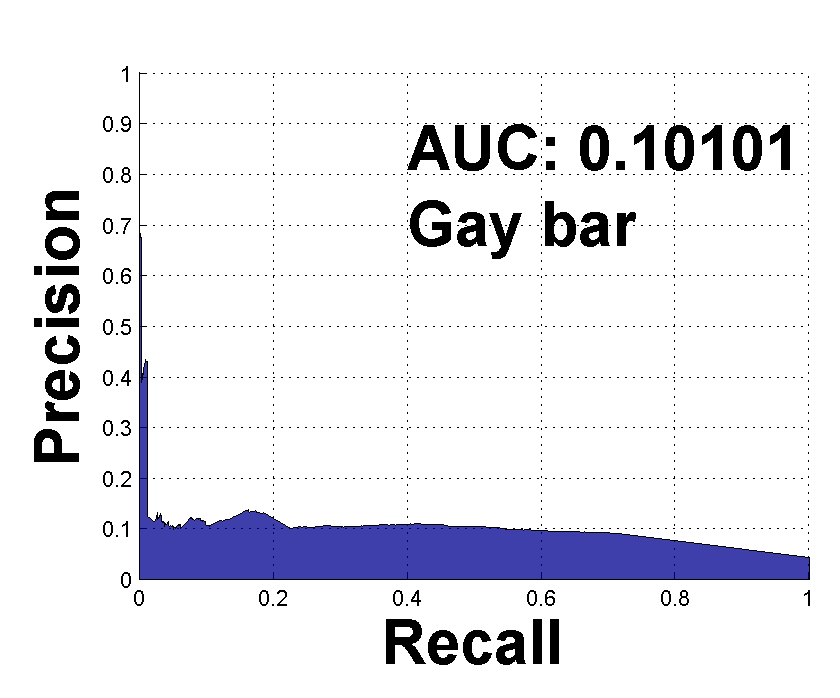
\includegraphics[width=1.5in]{fig/keyword/inf_gaybar_pr.eps}
\\
(a) & (b) \\

\hspace{-0.35cm}\includegraphics[width=1.5in]{fig/keyword/inf_stripclub_pr.eps}
&
\hspace{-0.35cm}\includegraphics[width=1.5in]{fig/keyword/inf_hospital_pr.eps}
\\
(c) & (d) \\
\end{tabular}
\caption{Precision-Recall curves for four sensitive keywords: (a) Church (b) Gay Bar (c) Strip Club (d) Hospital}
\label{fig:inference}
\end{figure}
As one can see, this attack is rarely effective, even in such extreme case where many user accounts have been compromised. The area under the curve is almost always very small. 
This turns out to be true even for locations that are sparse, as it is much more difficult to guess right when only a handful of users are visiting a rare location. 

This points to an interesting difference between inference in our scheme and de-anonymization attacks. While de-ano\-ny\-mi\-za\-tion attacks always benefit from sparsity since the data are present in a sanitized form, in our context, the attack does not always benefit from sparsity. This is because a minimum critical mass of typical behavior is needed in order to run inference. This shows that a proper choice of blacklist could potentially protect many locations, even as several accounts are compromised in the system. 

% Not sure where Bala wanted me to put this...

% More work remains to be done in this area. 
% One promising direction of study would be the effect of translating locations to keywords on k-anonymity in large traces.
% Another topic to be considered is trade-offs between time granularity and privacy.

\subsection{Attacks on Advertiser Revenue}
We now consider if advertisers can unfairly lose money to unscrupulous users of the system.
Because users are paid when they are accessed by advertisers, they have an incentive to view or click on many ads, even when they are not interested in the displayed products, to artificially boost their profile's value to derive more money from each click.
We label these activities ``user fraud." %different name??

% It is important to note that digital user fraud is really a special case of invalid traffic in online advertising.
User fraud is a special case of invalid traffic in online advertising.
According to Google's Ad Traffic Quality Resource Center, ``invalid traffic includes both clicks and impressions ... [that are] not the result of genuine user interest. This covers intentionally fraudulent traffic as well as accidental clicks and other mechanically generated traffic."\footnote{\url{www.google.com/ads/adtrafficquality/index.html}}
% This definition applies equally well to any clicks or impressions a user creates in order to game the system.
A request for an ad within our system is just like a request for an ad in the current ad ecosystem, but with some privacy-protecting filtering and potential additional location information.
Thus, previous techniques used to identify invalid traffic can be used to identify user fraud.
% Recently, there has been a variety of research on this subject.
There is a lot of recent research on this topic.
Dave et al propose methods to fingerprint click spam~\cite{clickspam}.
Haddadi uses ``bluff ads", ads designed to not appeal to humans and thus only be clicked by bots, to defeat click fraud~\cite{bluffad}.
Information on the structure of Google's click fraud detection system is available ~\cite{googleClick1}. %, ~\cite{laneGiftReport}.
Beyond academia, multiple startups exist that estimate the rates of click fraud,
such as Adometry, Visual IQ, and ClearSaleing~(%\footnote{
\url{www.adometry.com}, \url{www.visualiq.com}, \url{www.clearsaleing.com}
%}
).
% We first note that such a problem is only as difficult as that of standard click fraud on the web.
% The amount of money to show one impression of an ad on the internet is exceedingly low, meaning the amount of money a user can expect to get from viewing an impression in our system will also be low.
% Thus, we only need to worry about 

Additionally, it is easier to detect user fraud than traditional invalid traffic because location information is more constrained than web-browsing.
Users are physically constrained in how far they can travel in a certain period of time
and typically display periodic mobility patterns, returning to their homes at night and spending week days at work locations.
A more extreme use of physical constraints would be to use location tags; fingerprints extracted from ambient signals at a specific location at a specific time~\cite{NarayananTLHB11}.
These constraints can be used to filter out automated attacks on a system. 
For example, if a user appears to be traveling faster than is physically possible, we can remove them from the system or verify their accounts with a Captcha or phone call.
Because of these physical constraints, and because click fraud prevention techniques can easily be applied to our system, we believe that our system is no more vulnerable to gaming than current online advertising. 
% Although click fraud is considered an open problem by the research community, 
The ongoing viability of online advertising shows that our solution should likewise not be derailed by invalid traffic.

% Beyond digitally generated location fraud, 
Beyond automated attacks, users might ``physically" attack the system by simply going to a high value location in order to appear more valuable to an advertiser than they actually are.
Again, techniques to combat click fraud can be employed here.
Click fraud techniques must deal with situations in which users actually click links to unfairly gain money, a nice analogy to this form of attack.
Beyond this, traveling to a location takes significant time and effort and will likely be too costly to be a viable way of making money.

% Traveling to a location takes significant time and effort. Such time and effort has an opportunity cost. 
% In order to make such an attack worthwhile, the user would have to have a very valuable profile. We don't anticipate profiles having such a high value unless the user has made multiple purchases in the past, in which case the advertiser would be compensated appropriately.
% Finally, the market should help deal with these attacks. We believe that valuable profiles will be distinguishable from worthless ones. The market should then be able to appropriately price them. To aide in this distinction, some reputation scheme could be added on top of the user's profile. For example, a user could receive a rating based on how often they respond to advertising.

% Gaming of the system is certainly an issue and an area for future study. 
% However, we believe that such concerns are no more difficult than the current click fraud situation facing online advertising.
% Given that online advertising is a thriving field in spite of these concerns, we feel that gaming does not pose a disastrous risk to our system.

% \section{Related Work}
\label{sec:relwork}

%We have presented an economic solution to location privacy that we refer to as
%transactional location privacy. Our solution has a economic component that
%associates a value to each location disclosure and a systems component that 
%helps maintain privacy. 

%Lot of work has been done on the economics of information disclosure~\cite{Ghosh:2011jy, Cvrcek:2006vv, Danezis:2005wq}.
%Ghosh et al. discuss and analyze economic value of information as treated by differential privacy~\cite{Ghosh:2011jy}. 
%Our work is different in that we focus on location information and we stress releasing non-obfuscated, pure information, instead of adding noise to a release as differential privacy dictates. 
%We believe releasing raw data is crucial for any solution to be supported by web service providers. 
%Carrascal et al~\cite{Carrascal} utilized experience sampling to study how users value their personal information online.
%Danezis et al studied specifically the worth of location information from
%the perspective of users~\cite{Cvrcek:2006vv, Danezis:2005wq}.
%Our work seeks to create a market that determines a price for user data based on what companies are willing to pay and what consumers are willing to receive.
%% Our work is complementary as we develop a model to quantify how much location is worth from the perspective of ad-networks and aggregators.

Our work is part of a growing body of work that deals with privacy solutions that aim to reconcile the privacy concerns of users with the economic needs of `free' online web services and mobile applications~\cite{Guha:2011wj, guha:koi, Riederer:2011ta, Toubiana:2010tm}. 
Privad~\cite{Guha:2011wj} and Adnostic~\cite{Toubiana:2010tm} are browser based systems that enable behavioral targeting while ensuring users' PII is not leaked to ad-networks performing the targeting. 
Our focus in this paper is different -- we are concerned with location information on mobile devices. 
Koi~\cite{guha:koi} is a system developed to address location privacy by way of location matching -- applications and service providers pre-declare which locations they would be interested in and the device releases this information at those specified locations. 
Our solution is different, in that we have an economic component where application developers need to pay
to access the user at the specified location. 
In addition, neither the device nor applications have to be modified to use our solution. 
% We believe incentives of economic gains are much stronger to increase adoption of a privacy solution. 
Our work is closely related to transaction privacy~\cite{Riederer:2011ta}.
The difference is that we focus on location information for mobile devices and develop a keyword-based disclosure scheme.
% an economic model of location information to drive our market. 

% With less econ, this is deemphasized a bit...
% Bacelli et al~\cite{infocom:fb} authors propose models to quantify the economic value of various locations, with the specific example of proximity advertising in mind.
% With regards to the economic valuation of location information, the closest work to ours is the work by Bacelli et al~\cite{infocom:fb} where the authors propose models to
% This is similar to our proposal, in that we too focus on proximity advertising and are interested in real-time location information. 
% The main difference is that our approach is more empirically driven and much simpler with fewer assumptions. We rely on keywords associated with locations (derived from real data) and make no assumptions on how various businesses are distributed in a geographical region.  
% We focus more on intent, captured by frequency of visits to a location, to approximate interest in a location and the propensity to conduct a commercial transaction at that location.
% Bacelli et al rely on a set of interests of a user that are known to the model.

% \section{Conclusion}
\label{sec:conclusion}

The collection and monetization of location information has become a large concern. % for privacy advocates and regulatory bodies. 
The main contribution of this paper is the design and analysis of a solution for location privacy using economics.
Our solution is simple -- opt-in users decide which locations to reveal and only these locations are sold on an information market. 
Buyers pay to gain access to users at specified locations.
Locations are specified in keywords, a notion intuitive to both end users and advertisers.
Our solution relies on a privacy protection component that ensures that the location information the user chooses not to release will not be leaked, and also minimizes the linkage of the user's identity with the released information. 
Future research  directions on keyword-based disclosure may include reducing the role of the trusted third party, larger implementations, and a stronger economic analysis of the solution.
A few locations, at a cell level, have been shown to provide poor anonymity~\cite{de2013unique}.
An interesting open question is if keywords provide better k-anonymity.

% We find that in terms of the value of location information, very few locations (5\%) account for majority of the value.
% We find that potentially sensitive locations (as defined by sociological research) appear to be well distributed across locations sorted by popularity and profitability.
% Likewise, we find that the potential revenue of these sensitive locations is small compared to the total value generated from all locations. 
% This suggests a sweet-spot between location privacy and monetizing location information.
% We construct and deploy a small scale version of the system with real users, showing that our solution is indeed feasible.
% We observe their behaviors and lay the groundwork for future study.



\chapter{Location Data, Demographics, and Bias}
\label{chap:bias}
  \section{Demographic Mobility}
  \label{sec:bias}
  % Introduction

\subsection{Related Work}


\subsection{Completed Work}



\subsubsection{I Don’t Have a Photograph But You Can Have My Footprints}

\subsubsection{Scaling up the Census with Social Media}



  \section{Inferring Demographics from Social Media}
  \label{sec:demo}
  % Motivation, what this section is about
% Data collection
% Labeling schemes (include table)
% Face: Calibration plot and face to accuracy
% Location: Calibration plot and face to accuracy
% Scaling: Agreement plot
% Debiasing
% Conclusion.


% Motivation, what this section is about
In this section, we evaluate the feasibility of combining publicly available social media images and metadata (including location) with modern facial recognition techniques to conduct large scale demographic research.
We find that facial recognition can be used to label the gender and race of social media profiles with high precision and recall.
We further investigate factors that improve or hinder demographic labeling accuracy, showing a disparity between the accuracy of labelings of profiles of racial majority and minorities.
% We conclude with ideas for future improvements and research.
% \end{abstract}

% Data collection
% Fig: Table of data
\begin{table}[h]
\centering
\begin{tabular}{l r r r r}
\emph{Name} & \emph{Users} & \emph{Photos} & \emph{Geotagged} & \emph{Prosograms} \\ \hline
Full & 260,389 & 115M & 16.5M & \\ 
Face & 4,166 & 1.5M & 64.6k & 322k \\ 
Labeled & 172 & 16,655 & 5,489 & 5,272 \\ 
\end{tabular}
\caption{Overview of Datasets \label{tab:data}}
\end{table}

For our research, we used a large dataset of Instagram photo metadata obtained through Instagram's API under the Terms of Service.
Similar to the work described in~\chap{sec:bias}, we gathered the metadata (such as time of photo, URL of image, tags, location, etc.) for all photographs of a ``root" user, Kevin Systrom, the founder of Instagram, and then collected the user IDs of users who had commented on or ``liked" his photos, gathered their metadata, and repeating this process in a random outward searching manner.
This process resulted in over 115 million photos on over 260,000 profiles.
A summary of this data (and derived data described in subsequent sections) is displayed in Table~\ref{tab:data}.

For subsets of profiles, we gathered additional information.
For all photos, we included geographic information when available.
For a randomly selected subset, we ran a publicly available face recognition API\footnote{\url{faceplusplus.com}} on a users first 100 Instagram images.
In addition to recognizing faces within images, Face++ labels race from \{White, Black, Asian\} with a \emph{confidence score} 0-100 and gender from \{Male, Female\} with a \emph{confidence score} 0-100.
For a smaller subset of users, two research assistants labeled a randomly selected subset for the collected profiles for gender and race, with 98.8\% agreement on gender and 85.5\% agreement on race, with the labels consistent with the Face++ set.


% Labeling schemes (include table)
% Fig: Table of labeling techniques
\begin{table}[h]
\centering
\begin{tabular}{l l l l}
\emph{Name} & \emph{Cost} & \emph{Speed} & \emph{Accuracy} \\ \hline
Manual & Expensive & Moderate & High \\ 
Face Recognition & Free / Cheap & Slow & Moderate \\ 
Census & Free & Fast & Low \\ 
\end{tabular}
\caption{Demographic Labeling Techniques \label{tab:techniques}}
\end{table}

There are many different ways to go from the ``raw" signal of social media to clean labels of demographics.
In this section, we consider three, with the relative comparison of the costs and benefits displayed in Table~\ref{tab:techniques}.
\textbf{Manually} labeling profiles using humans to examine each one will result in the highest accuracy, but will have high monetary costs.
Time for labeling can be moderate if done in parallel with many labels, and much slower if done serially by few individuals. 
\textbf{Face recognition} can provide a valuable signal for gender or race based on image analysis.
Depending on the implementation, this can be very cheap, as it is bounded by computation.
However, face recognition algorithms are imperfect and may exhibit statistical bias towards different groups, and may be slow if bounded by API services or computation.
Finally, using \textbf{location data}, as described in \chap{sec:bias}, can be incredibly fast and cheap, but will have low accuracy depending on prediction task, location granularity, and other factors.
We next explore in detail the accuracy of each of these methods.
For the sake of brevity, these results include only information on predicting US Census Race classifications, but we have additional work on binray gender classification available as well.

% Location: Calibration plot and face to accuracy
% Fig: confusion matrix
% \begin{wrapfigure}{R}{0.5\textwidth}
\begin{table}[h]
\centering
\label{tab:cm_race_loc}
\begin{tabular}{l r r}
\emph{Race} & \emph{Predicted Minority} & \emph{Predicted White} \\ \hline
Minority & 8 & 31 \\
White & 5 & 88 \\
\end{tabular}
\caption{Location-Based Race Labeling Confusion Matrix}
\end{table}
% \end{wrapfigure}

\begin{wrapfigure}{R}{0.48\textwidth}
% \begin{figure}[h]
  \centering
  % \begin{minipage}{\halfwidth}
    % \centering
    \includegraphics[width=0.48\linewidth]{fig/census/calibration_race_loc-eps-converted-to.pdf}
  % \end{minipage}
  % \begin{minipage}{\halfwidth}
    % \centering
    \includegraphics[width=0.48\linewidth]{fig/census/locs_v_accuracy_race_labeled-eps-converted-to.pdf}
  % \end{minipage}
  \caption{Location Prediction: Calibration and data amount to accuracy of race prediction.\label{fig:accuracy_race_loc}}
% \end{figure}
\end{wrapfigure}

Based on previous results, we expected location to provide more of a signal for race than for gender.
Census tracts in the United States show a much more skewed distribution in regards to race than to gender, with the majority of tracts being heavily Caucasian, but with a sizeable fraction of tracts (>6\%) having smaller than 20\% Caucasian. 
On a baseline of 70.4\% white users (including Hispanics), using the average percentage of census tracts visited predicted 73.4\% of users' races.
Our figures show that there is some weak signal in terms of ROC.
The algorithm is well calibrated but again does not make strong predictions on most users.
Accuracy is very poor on minorities, compared to Whites, and after an initial jump in accuracy after ten locations, is not greatly affected by the number of geotagged in the users profile.
The number of locations used seems to have little effect on accuracy, which remains low for minorities and high for Whites.


% Face: Calibration plot and face to accuracy

\begin{table}[h]
\centering
\begin{tabular}{l r r}
\emph{Race} & \emph{Labeled Minority} & \emph{Labeled White} \\ \hline
Minority & 33 & 11 \\
White & 4 & 97 \\
\end{tabular}
\caption{Content-Based Race Labeling Confusion Matrix\label{tab:cm_race_face}}
\end{table}

\begin{wrapfigure}{R}{0.5\textwidth}
% \begin{figure}[h]
  \centering
  % \begin{minipage}{\halfwidth}
    % \centering
    \includegraphics[width=0.48\linewidth]{fig/census/calibration_race_face-eps-converted-to.pdf}
  % \end{minipage}
  % \begin{minipage}{\halfwidth}
    % \centering
    \includegraphics[width=0.48\linewidth]{fig/census/faces_v_accuracy_race_labeled-eps-converted-to.pdf}
  % \end{minipage}
  \caption{Face prediction: Calibration and data amount to accuracy of race prediction.\label{fig:accuracy_race_face}}
% \end{figure}
\end{wrapfigure}

In Fig.~\ref{fig:accuracy_race_face}, we see that the algorithm is underconfident, outputting a lower probability than warranted when predicting if a user is white.
An important aspect of demographic labeling is considering issues of the digital divide or disparate impact.
In the rightmost plot of Fig.~\ref{fig:accuracy_race_face}, we see that accuracy is much lower on minorities than it is on White users.
Errors seem biased towards underrepresentation of minority groups.
This could have consequences as the algorithmics introduce a hegemonic factor in favor the majority.
% In section~\ref{sec:scaling} we discuss a principled technique for maintaining equal accuracy rates across groups while maintaining high overall accuracy.

% Scaling: Agreement plot
% \begin{figure}[h]
%   \centering
%   \begin{minipage}{\halfwidth}
%     \centering
%     \includegraphics[width=\linewidth]{fig/census/faces_v_accuracy_gender_large-eps-converted-to.pdf}
%   \end{minipage}
%   \begin{minipage}{\halfwidth}
\begin{wrapfigure}{R}{0.33\textwidth}
  \centering
  \includegraphics[width=\linewidth]{fig/census/faces_v_accuracy_race_large-eps-converted-to.pdf}
  \caption{Agreement as data increases}
  % \end{minipage}
  \label{fig:faces_v_accuracy_large}
\end{wrapfigure}
% \end{figure}

In both our face recognition and location-based labeling methods, as the number of photos used increases, the impact of one individual photo goes down.
We therefore should expect that at some point we should observe ``diminishing returns" in terms of the amount of data collected.
In other words, we do not need to crawl all photos of a profile in order to know what our algorithm will label it.
We investigate this idea in Figure~\ref{fig:faces_v_accuracy_large}.

We first gather all face data for each user, labeling their entire profile.
Using all of the data, we a label a profile for gender and race using our algorithms.
For each user, we then restrict the data input to the algorithm to a smaller subset and record our prediction.
We repeat this process, gradually decreasing the amount of data supplied to the algorithm until we only give one photo.
For each number of prosograms used, we calculated what percentage of users have the same label as their label from the full labeling.
We see in the left figure that if we used just 1 picture, the output of our algorithm would agree with the full data about 75\% of the time, and this is the same for both male and female profiles.
After 100 prosograms, very few profiles will change their label.
This suggests that for gender, we need only collect the first 100 prosograms to get a highly accurate estimate on our algorithm's result on the entire user profile data.

We observe similar behavior in the race dataset, depicted in the right side of Fig~\ref{fig:faces_v_accuracy_large}.
After 100 photos, our algorithm is similarly unlikely to change its label.
However, in contrast to gender, we see divergent levels of agreement for our two labels, with profiles eventually labeled minority more likely to disagree than white profiles.
This points to a potential bias in either the data or in the labeling algorithm, again suggesting that care must be taken in order to achieve balanced error rates across classifications.

% Debiasing
\paragraph{Debiasing}
Oftentimes, scientists might choose to optimize accuracy or a class-centric metric like F1.
However, choosing to optimize for metrics focused on one class (such as Female or White) can cause systemic biases to appear, as accuracy improves for one class but is ignored for another.
This can be of particular in demographic labeling, where we would like to have proper representation of multiple groups.
For example, when using the threshold of 0.5, we see large disparities between White and Minority labels as the data scales, as appears in Figures~\ref{fig:accuracy_race_loc} and~\ref{fig:accuracy_race_face}.

\begin{wrapfigure}{R}{0.48\textwidth}
  \centering
    \includegraphics[width=0.48\linewidth]{fig/census/locs_v_accuracy_race_labeled_ber-eps-converted-to.pdf}
    \includegraphics[width=0.48\linewidth]{fig/census/faces_v_accuracy_race_labeled_ber-eps-converted-to.pdf}
  \caption{Location or faces vs. accuracy, with a choice of threshold determine by Balanced Error Rate.\label{fig:debias}}
\end{wrapfigure}

% \begin{wrapfigure}[R]{0.5\textwidth}
%   \centering
% % \begin{figure}[h]
%   % \begin{minipage}{\halfwidth}
%     % \centering
%     \includegraphics[width=0.48\linewidth]{fig/census/locs_v_accuracy_race_labeled_ber-eps-converted-to.pdf}
%   % \end{minipage}
%   % \begin{minipage}{\halfwidth}
%     % \centering
%     \includegraphics[width=0.48\linewidth]{fig/census/faces_v_accuracy_race_labeled_ber-eps-converted-to.pdf}
%   % \end{minipage}
%   \caption{Location or faces vs. accuracy, with a choice of threshold determine by Balanced Error Rate.\label{fig:debias}}
% % \end{figure}
% \end{wrapfigure}

Instead of optimizing for accuracy or F1, one method to insure equal levels of error in both classes is to instead optimize for Balanced Error Rate (BER).
Balanced error rate is simply an average of the error in each class, that is, 
$\frac{1}{2}\epsilon_1 + \frac{1}{2}\epsilon_2$, where $\epsilon_1$ and $\epsilon_2$ represent the error in class 1 and 2 (e.g. Female and Male, or White and Minority).

% Interpret results
Figure~\ref{fig:debias} shows how accuracy scales with more data for race when using a threshold determined by optimal BER. 
The thresholds were 0.58 for faces and 0.67 for location.
Comparing with Figures~\ref{fig:faces_v_accuracy_race_labeled} and~\ref{fig:locs_v_accuracy_race_labeled_1}, we see lines much closer together, indicating error rates much closer to one another than previously.
Choosing another metric, such as F1, indeed leads to problems in the example of location.
Here, a threshold of 0.33 is chosen.
Although this gives an accuracy of 100\% for White, it affords only 10.3\% accuracy for minorities.

Using BER as a metric in training can help us in designing algorithms that will fairly label users when conducting demographic research.
Such techniques are especially important when being used in unsupervised settings, where algorithmic bias can impact accuracy on a large scale.


% Conclusion...





% \textbf{Introduction} \\
% The great wealth of publicly available, online social networking data has been a boon to demographic research due to its richness and scale.
% Never before has such an amount of human behavioral data been easily obtained and analyzed.
% However, before this data can be used to study demographics, each user must be labeled with demographic categorizations. 
% This poses a particular challenge in many online social networking (OSN) sites which often do not display or even obtain the demographic information of its users.

% To meet this need, researchers in the past have tried a variety of techniques.
% Manual labeling by individually investigating each profile is costly in terms of time, effort, and money.
% Some studies have relied on data provided by marketing companies or data aggregators~\cite{Goel:2012ut, biinferring}.
% Due to cost and issues of reproducibility, these sources of data are not available to all researchers.

% To improve the scale of labeling while keeping costs low, researchers have used automated techniques which range in complexity.
% For example, researchers have compared public names to lists of gender and ethnicity for those names~\cite{mislove-2011-twitter, ICWSM101534}.
% Others have run simple algorithms on location data~\cite{riederer2015cosn} or more sophisticated techniques that incorporate text posted and the structure of a user's social network~\cite{ICWSM112886, pennacchiotti2011democrats}.
% These techniques offer some promise but often are not very robust and may not be applicable to OSNs with little textual interaction, such as Instagram.

% % TODO: This doesn't really fit.
% Researchers that use these automated tools for labeling must be wary of introducing algorithmic bias.
% As argued in~\cite{Selbst:2014wi}, data mining can lead to biased results.
% Algorithms that have disparate accuracies in demographic labeling could cause erroneous or biased results.

% In the past, computational vision has not been an effective technique for labeling the demographics of social media users, due to three issues: (1) CV algorithms being too slow, (2) CV algorithms having low accuracy, (3) a lack of publicly available and uniformly popular photographs as data.
% However, in recent years, face recognition tools have improved to become both highly accurate and efficient.
% Additionally, the social network Instagram has made image-sharing a ubiquitous activity across most of the developed and much of the developing world.

% Instagram is an interesting social network to study for a variety of reasons.
% With over 400 million users at the time of writing, over 5\% of the world's population user Instagram.
% A quarter of these users are based inside the United States, meaning that nearly 1 in 3 United States citizens uses Instagram~\cite{igstats}.
% Beyond its scale, Instagram is interesting for its content.
% Photographs are extremely rich, capturing information on all sorts of human activities and interactions.
% Although images can be more difficult to analyze than text, the research community has begun to study Instagram behavior~\cite{hu2014we, bakhshi2014faces} and even selifes~\cite{souza2015dawn}.

% In this paper, we show that a popular face recognition API can be used to scalably and accurately learn the gender and race of Instagram users.
% We use a dataset of 200 Instagram profiles, labeled for gender and race, to analyze the practicality and accuracy of facial recognition, achieveing 86\% accuracy for gender and 82\% accuracy for race in a limited setting.
% We additionally explore the accuracy of labeling different demographics as the amount of data increases, showing some concerns about algorithmic bias.
% We conclude with ideas for future work.

% \textbf{Data} \\
% \textbf{Collection} \\
% We used a subset of the Instagram data collected in~\cite{riederer2015cosn}.
% In this paper, the authors gathered the metadata (such as time of photo, URL of image, tags, location, etc.) for all photographs of a ``root" user, Kevin Systrom, the founder of Instagram.
% They then collected the user IDs of users who had commented or liked his photos, gathered their metadata, and repeated this process.
% A subset of these users were then selected based on geography-- only users with more than half of their photographs taken in Los Angeles or New York were kept.

% Two research assistants labeled a randomly selected subset of 200 of these profiles for gender and race.
% After filtering for private, deleted, or business profiles, 172 profiles remained.
% For gender, the labelers selected from male, female, or other.
% In practice, only the male or female categories ended up being used.
% For race, a subset of the United States Census categories were used: White, Black, Hispanic, Asian, and other.
% The labelers agreed on gender for 170 of the profiles and for race on 147.
% The process resulted in 76 profiles as Male and 94 as Female.
% For race, 75 were labeled White, 28 as Hispanic, 27 as Black, 16 as Asian, and 1 as other.

% Our next step was to recognize and label faces present in these Instagram users' profiles using computer vision.
% For this task, we used Face++~\cite{faceplusplus}, a popular API with reported high degress of accuracy~\cite{bakhshi2014faces}.
% In addition to recognizing faces within images, Face++ labels race from {White, Black, Asian} with a \emph{confidence score} 0-100, gender from {Male, Female} with a \emph{confidence score} 0-100.

% For each user in this data set, we gathered the metadata of the first 100 Instagram photos.
% Each image was then analyzed with the Face++ API.
% Face++ only requires that a URL to an image is passed to it.
% Therefore, this methodology does \emph{not} require that any images are downloaded, uploaded, or even viewed by a human labeler.
% Note that not every photo on Instagram has a face in it, and some have more than one.

% This resulted in 170 distinct users with at least one or more face present in their photos.
% We obtained 5,272 photos and depicting 12,143 faces. 
% Additionally, for each user, we passed the URLs for their profile pictures.
% A total of 70 users had profile pictures in which Face++ could detect a face.
% 73 faces were found: 2 profiles pictures had 2 faces in them.

% \textbf{Description}


% \begin{figure}[t]
%   \centering
%   \begin{subfigure}[b]{.21\textwidth}
%     \centering
%     \includegraphics[width=\linewidth]{fig/census/face_cdf_gender.eps}
%     \caption{}
%     \label{fig:face_cdf_gender}
%   \end{subfigure}
%   \begin{subfigure}[b]{.21\textwidth}
%     \centering
%     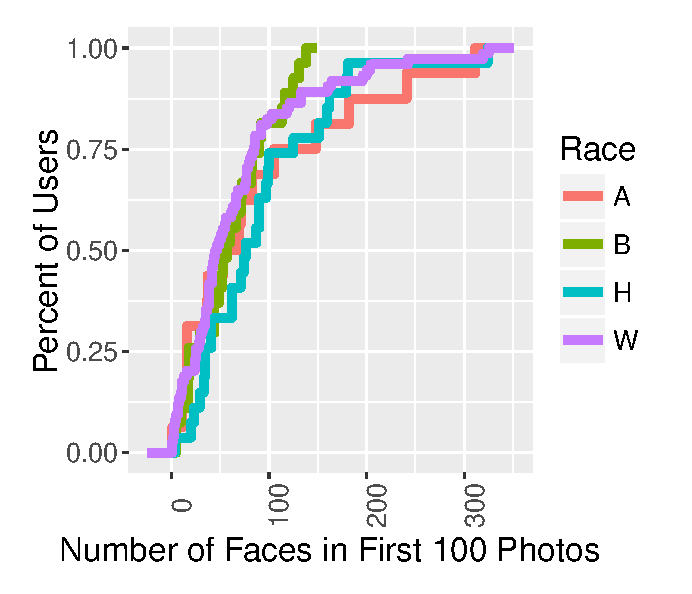
\includegraphics[width=\linewidth]{fig/census/face_cdf_race.eps}
%     \caption{}
%     \label{fig:face_cdf_race}
%   \end{subfigure}
%   \caption{}
%   \label{fig:face_cdf}
% \end{figure}

% \begin{figure}[t]
%   \centering
%   \begin{subfigure}[b]{.21\textwidth}
%     \centering
%     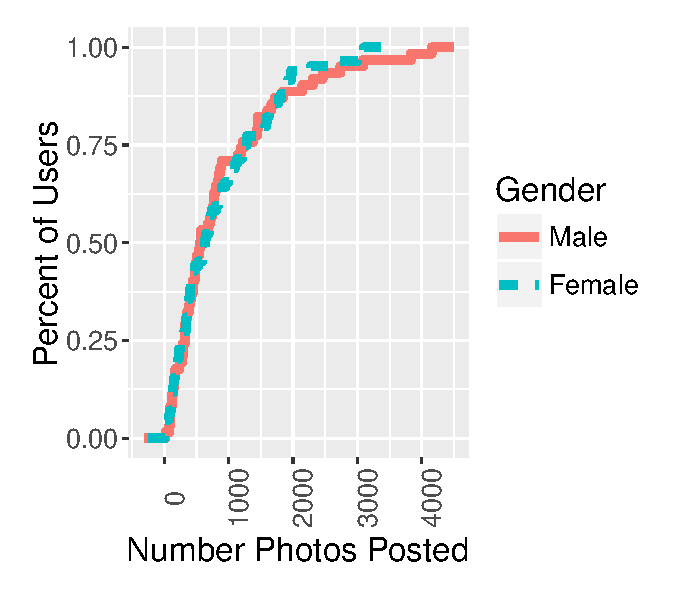
\includegraphics[width=\linewidth]{fig/census/numphoto_cdf_gender.eps}
%     \caption{}
%     \label{fig:numphoto_cdf_gender}
%   \end{subfigure}
%   \begin{subfigure}[b]{.21\textwidth}
%     \centering
%     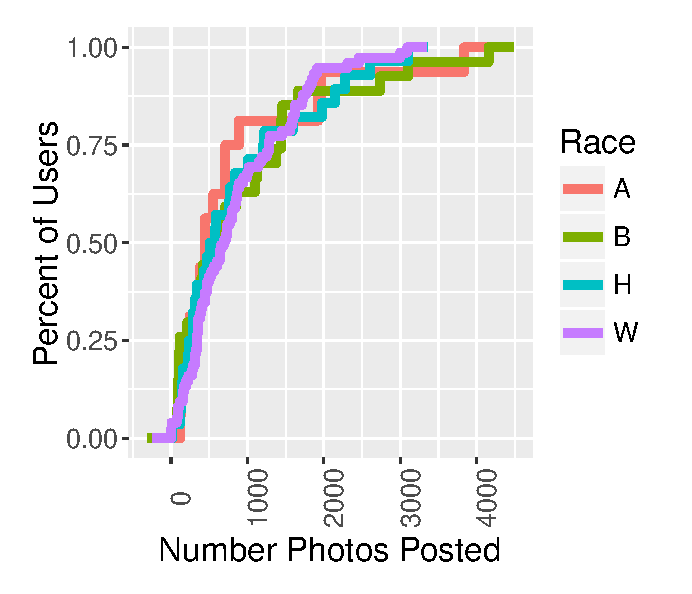
\includegraphics[width=\linewidth]{fig/census/numphoto_cdf_race.eps}
%     \caption{}
%     \label{fig:numphoto_cdf_race}
%   \end{subfigure}
%   \caption{}
%   \label{fig:numphoto_cdf}
% \end{figure}


% \begin{figure}[t]
%   \centering
%   \begin{subfigure}[b]{.21\textwidth}
%     \centering
%     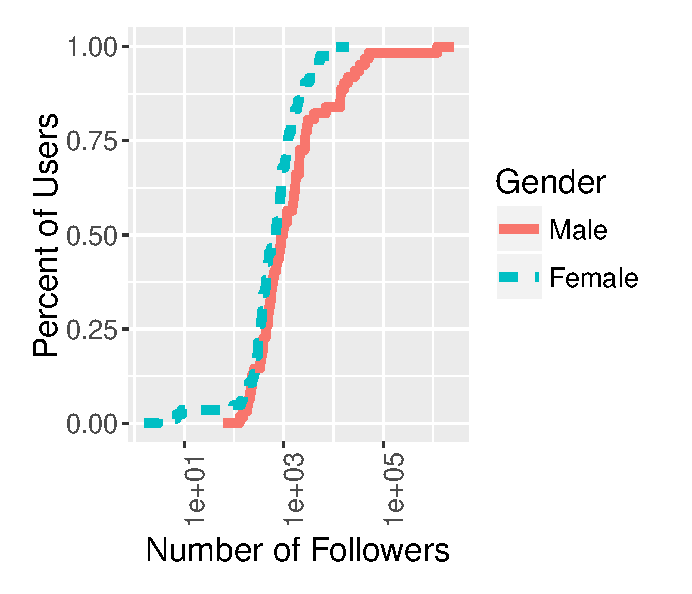
\includegraphics[width=\linewidth]{fig/census/followers_cdf_gender.eps}
%     \caption{}
%     \label{fig:followers_cdf_gender}
%   \end{subfigure}
%   \begin{subfigure}[b]{.21\textwidth}
%     \centering
%     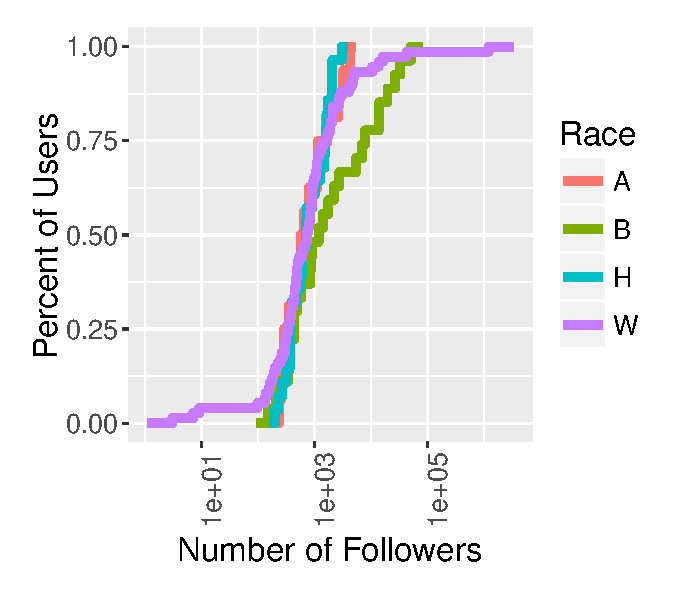
\includegraphics[width=\linewidth]{fig/census/followers_cdf_race.eps}
%     \caption{}
%     \label{fig:followers_cdf_race}
%   \end{subfigure}

%   \begin{subfigure}[b]{.21\textwidth}
%     \centering
%     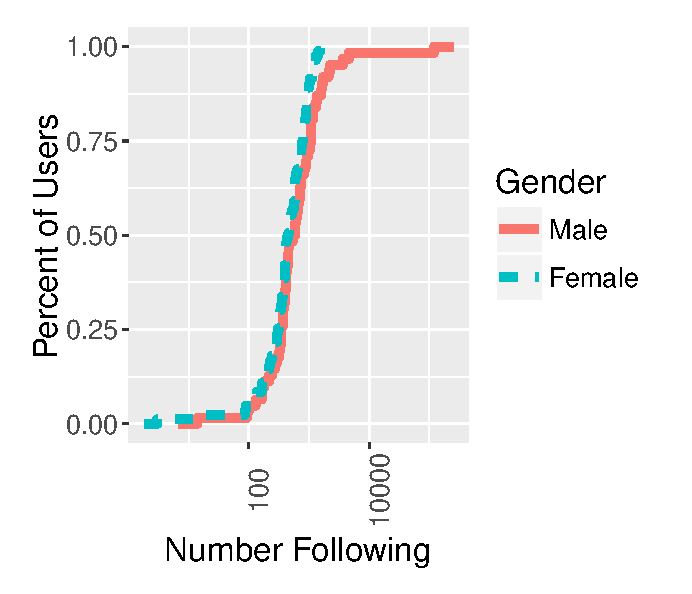
\includegraphics[width=\linewidth]{fig/census/following_cdf_gender.eps}
%     \caption{}
%     \label{fig:following_cdf_gender}
%   \end{subfigure}
%   \begin{subfigure}[b]{.21\textwidth}
%     \centering
%     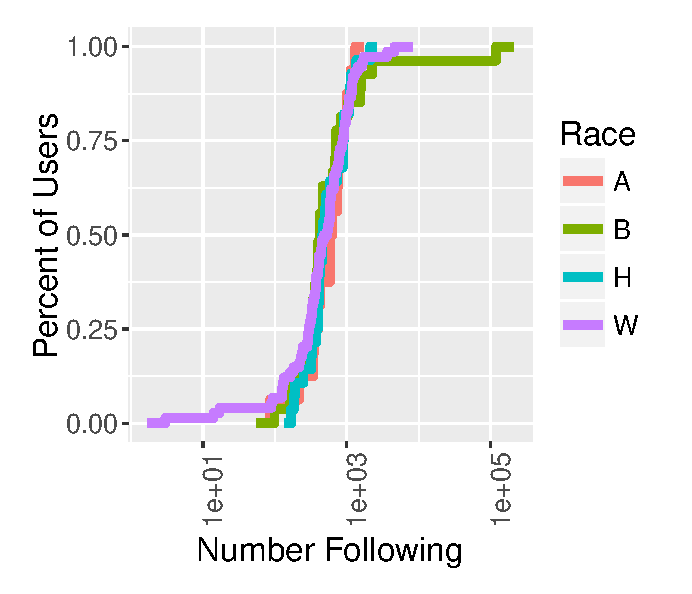
\includegraphics[width=\linewidth]{fig/census/following_cdf_race.eps}
%     \caption{}
%     \label{fig:following_cdf_race}
%   \end{subfigure}
%   \caption{}
%   \label{fig:follow_cdf}
% \end{figure}

% We next compared several Instagram behaviors by demographic.
% Figure~\ref{fig:face_cdf_gender} shows that women in our dataset typically have more faces in their photographs than men.
% There appears to be more parity in number of faces for each of the considered racial groups, with Hispanics and Asians displaying slightly more faces in their photos.

% We examine potential differences in the total number of photos posted by a user to their account in Figure~\ref{fig:numphoto_cdf}.
% There does not appear to be a great difference for any particular group.

% We investigate the relationship between gender, race, and following behavior in Figure~\ref{fig:follow_cdf} .
% Instagram has a directional follower relationship, akin to that of Twitter.
% If a user, Alice, follows Bob, it means that Alice will see updates from Bob in her feed.
% Bob, however, will not see updates from Alice unless he decides to follow her.
% Figures~\ref{fig:followers_cdf_gender} and~\ref{fig:following_cdf_gender} show differences in following behavior within our dataset for gender. 
% It appears that men have more followers, and follow slightly more people.

% In Figures~\ref{fig:followers_cdf_race} and~\ref{fig:following_cdf_race}, we see can make a few observations for following behavior among race in our dataset.
% First, we see that the upper 50\% of Black users in our dataset have more followers than other groups, except for at the very top percentiles, where White users dominate.
% At the highest percentiles, Black users \emph{follow} the most people.
% % TODO: mention Black Twitter...
% % http://www.slate.com/articles/technology/technology/2010/08/how_black_people_use_twitter.html
% % Maybe http://dl.acm.org/citation.cfm?id=1963503
% % duggan and smith: demo of key social networking platforms



% \textbf{Methodology}
% % Recognizing and labeling the faces present in each photo does not definitively tell us the gender or race of the user profile. 
% The face recognition software only works at the level of a single photograph.
% % This does not tell us the race or gender of the user on which these photographs appear.
% We thus need to use an algorithm to go from the data of each picture to labeling an entire profile.
% We rely on one main assumption: the owner of profile will appear in more photos than any other individual.

% This assumption led us to test several different algorithms: 
% \begin{itemize}
% \item \textbf{Majority rule}: Count each face as a vote. 
%   Profile is labeled with the gender (or race) with the most votes.
% \item \textbf{Weighted majority rule}: Count each face as a vote.
%   However, a face now gets as many votes as the confidence score.
%   Thus, faces with lower confidence get lower weight.
%   Profile is labeled with the gender (or race) with the most votes.
% \item \textbf{Profile picture}: We simply take the result of the profile picture labeling.
% \end{itemize}

% Additionally, we applied a ``face weight" correction to all of these.
% In a photo with three faces, only one of these faces could be the user.
% It therefore might make sense to weight each face in this photo lower than in a photo with one face.
% The face weight (fw) correction does just this, multiplying the weight of photo by the inverse of the number of faces in that photograph.
% In our original example, the weight of each of the three faces would be multiplied by one third.
% This is equivalent to averaging the gender or race (potentially with confidence scores) of all users in a photograph.


% \textbf{Results}

% \textbf{Gender}
% Our human labelers categorized 76 profiles as Male and 94 as Female.
% Running our three algorithms with and without the face weight correction, we obtained the following results:
% \begin{itemize}
% \item \textbf{Majority rule}: 85.1\%
% \item \textbf{Weighted majority rule}: 85.7\%
% \item \textbf{Majority Rule, FW}: 86.9\%
% \item \textbf{Weighted Majority Rule, FW}: 87.5\%
% \item \textbf{Profile picture}: 86.3\%
% \end{itemize}

% We observe that using the face weight correction improves the results for both algorithms.
% Although profile pictures provide accurate information, only 70 out of 170 of these users had a profile picture that included a face.
% For the remainder of this section, we will focus on the highest accuracy algorithm, weighted majority rule with FW.
% A feature of this algorithm is that it outputs a probability for each user, enabling us to analyze the performance in more detail.
% % \begin{figure}[!tbp]
% %   \centering
% %   \begin{minipage}[b]{0.4\textwidth}
% %     \includegraphics[width=\textwidth]{flower1.jpg}
% %     \caption{Flower one.}
% %   \end{minipage}
% %   \hfill
% %   \begin{minipage}[b]{0.4\textwidth}
% %     \includegraphics[width=\textwidth]{flower2.jpg}
% %     \caption{Flower two.}
% %   \end{minipage}
% % \end{figure}

% \begin{figure}[h]
%   \centering
%   \begin{minipage}{.21\textwidth}
%     \centering
%     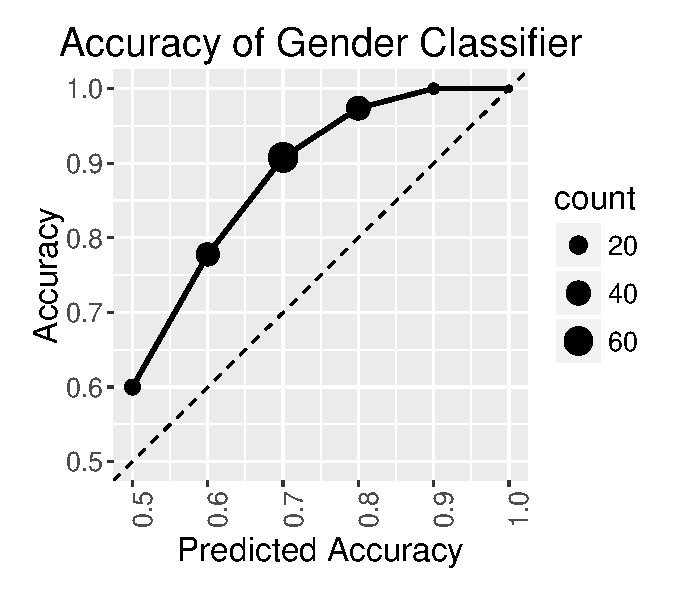
\includegraphics[width=\linewidth]{fig/census/accuracy_gender.eps}
%     \caption{Predicted accuracy versus actual accuracy }
%     \label{fig:accuracy_gender}
%   \end{minipage}
%   \begin{minipage}{.21\textwidth}
%     \centering
%     \includegraphics[width=\linewidth]{fig/census/roc_gender.eps}
%     \caption{True positive versus false positive rate when labeling at various threshold levels.}
%     \label{fig:roc_gender}
%   \end{minipage}
%   \caption{}
%   \label{fig:accuracy_gender_all}
% \end{figure}

% \begin{figure}[h]
%   \centering
%   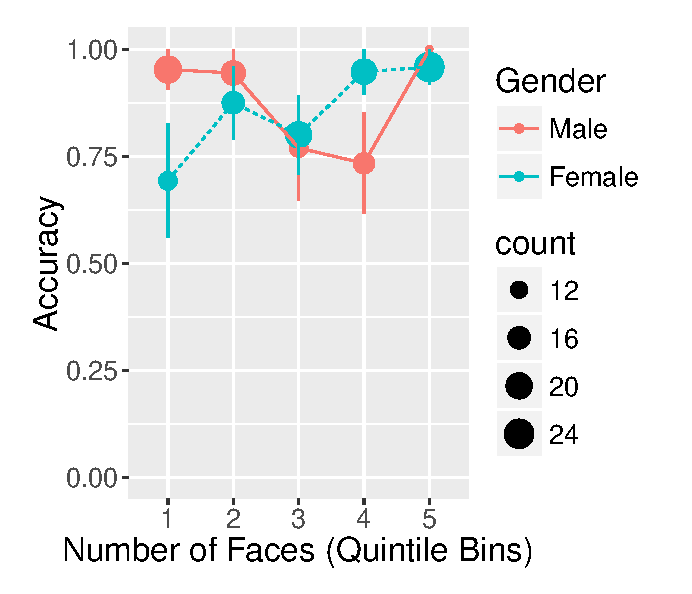
\includegraphics[width=.5\linewidth]{fig/census/facebin_gender.eps}
%   \caption{Number of faces detected in first 100 photos vs. accuracy, by gender}
%   \label{fig:facebin_gender}
% \end{figure}
% % TODO: add the boxplot thing in here, just because this looks bad right now

% In Fig.~\ref{fig:accuracy_gender}, we group individuals on how what our algorithm predicts is the likelihood that that individual is female, and plot the accuracy within each group.
% This shows us how well calibrated our algorithm is; if the output probability estimates are perfectly accurate, then half of the users with estimate 50\% should be female, and this plot should align on the 1:1 line.
% Instead, we see that the line is above the diagonal, meaning our accuracy estimate is actually an underestimate.
% Most likely, we could incorporate a prior probability into our algorithm to make it better calibrated.

% In Fig.~\ref{fig:roc_gender}, we plot an ROC curve, showing the trade-off between accurate and inaccurate labelings when using a threshold on the algorithm's output probability.
% For example, if we label as female all users with a probability of female over 60\%, around 75\% of female users would be correctly labeled, and we would exclude properly all but around 7\% of males.

% In Fig.~\ref{fig:facebin_gender}, we observe that for users labeled female, as more faces are detected in their profiles, accuracy increases.
% Perhaps counterintuitively, we see a dip for men, where male users with the 40-80\% most faces have much lower accuracy those in the bottom two quintiles, the bottom 40\%.
% One possible hypothesis to explain this is that as some users add more faces, they will start to add a larger diversity of faces.
% When this diversity increases, accuracy may decrease.
% We leave the question of whether this is the mechanism open for later work.


% \textbf{Race} \\

% For race, 75 users were labeled White, 28 as Hispanic, 27 as Black, 16 as Asian, and 1 as other.
% However, Face++ only labels users as Asian, Black, or White and will therefore always be incorrect on any of our users categorized as Hispanic or ``Other".
% Thus, we'll present results both for all users, and for the reduced set of users labeled manually by our research assistants as Asian, Black, or White (``filtered").
% Running our algorithms with and without the face weight correction, we obtained the following results:
% \begin{itemize}
% \item \textbf{Majority rule}: 64.4\% (all) 79.3\% (filtered)
% \item \textbf{Weighted majority rule}: 66.2\% (all) 82.1\% (filtered)
% \item \textbf{Majority Rule, FW}: 66.4\% 82.2\% (filtered)
% \item \textbf{Weighted Majority Rule, FW}: 66.2\% (all), 82.1\% (filtered)
% \item \textbf{Profile picture}: 57.1\% (all), 71.1\% (filtered)
% \end{itemize}

% On the users for which we have some hope of accuracy, the best algorithm achieves 82.2\% accuracy.
% For the remainder of this section, we will constrain our results to the Weighted Majority algorithm, FW, due to the probabilities that it outputs and its nearly identital performance to the next best algorithm.
% Additionally, we will look at some labelings as a binary classification problem between White users and Minority users.

% % TODO: fix titles here
% \begin{figure}[h]
%   \centering
%   \begin{minipage}{.21\textwidth}
%     \centering
%     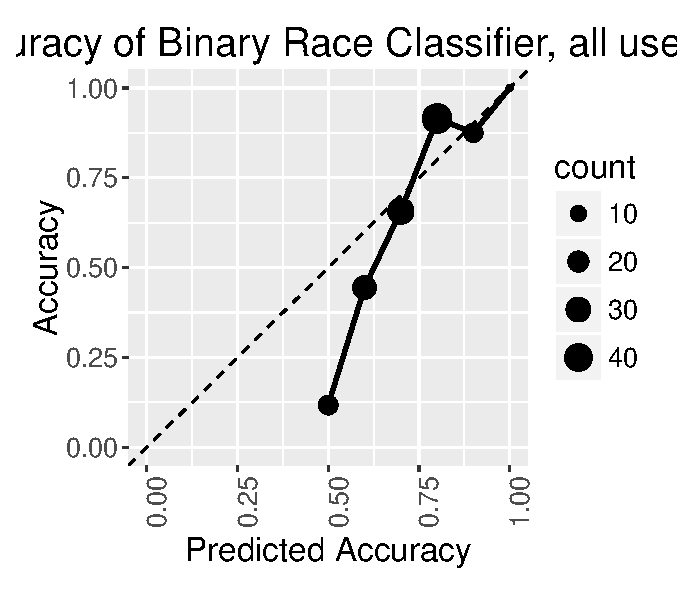
\includegraphics[width=\linewidth]{fig/census/accuracy_race_all.eps}
%     % \caption{Predicted accuracy versus actual accuracy }
%     \label{fig:accuracy_race_all}
%   \end{minipage}
%   \begin{minipage}{.21\textwidth}
%     \centering
%     \includegraphics[width=\linewidth]{fig/census/accuracy_race_filtered.eps}
%     % \caption{True positive versus false positive rate when labeling at various threshold levels.}
%     \label{fig:accuracy_race_filtered}
%   \end{minipage}
%   % \caption{}
%   \label{fig:accuracy_race}
% \end{figure}

% \begin{figure}[h]
%   \centering
%   \begin{minipage}{.21\textwidth}
%     \centering
%     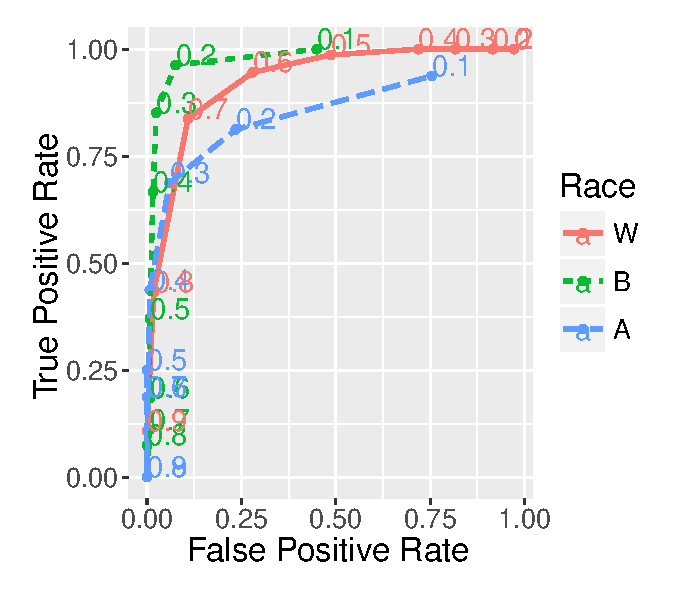
\includegraphics[width=\linewidth]{fig/census/roc_race.eps}
%     % \caption{Predicted accuracy versus actual accuracy }
%     \label{fig:roc_race}
%   \end{minipage}
%   \begin{minipage}{.21\textwidth}
%     \centering
%     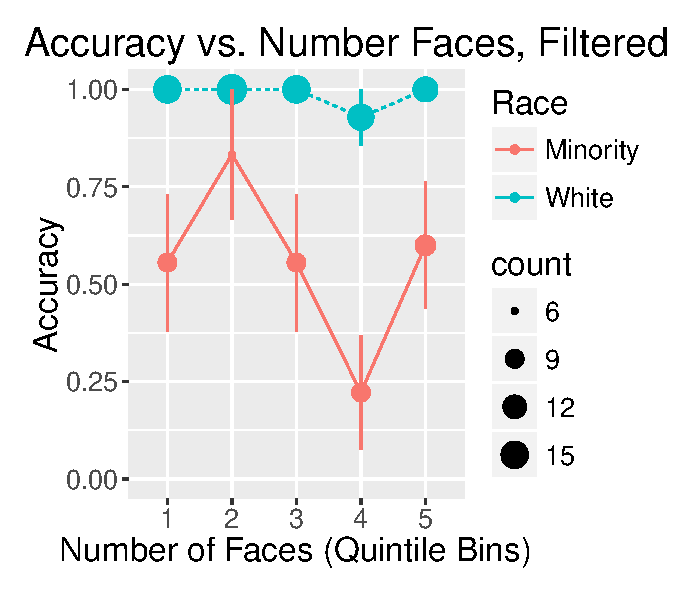
\includegraphics[width=\linewidth]{fig/census/facebin_race_filtered.eps}
%     % \caption{True positive versus false positive rate when labeling at various threshold levels.}
%     \label{fig:facebin_race_filtered}
%   \end{minipage}
%   \caption{}
%   \label{fig:more_race}
% \end{figure}

% Based on Fig.~\ref{fig:accuracy_race}, the algorithm does not appear to be well-calibrated, both in being overconfident in the users with low probability estimations, and being underconfident in users with higher estimates.

% An important aspect of demographic labeling is considering issues of the digital divide or disparate impact.
% In Fig.~\ref{fig:more_race}, we see that accuracy is much lower on minorities than it is on White users.
% Again, we see a lowering of accuracy as the number of faces increases, akin to the dip in accuracy Male users show in Fig.~\ref{fig:facebin_gender}.

% \textbf{Discussion} \\
% Among our dataset, we see some examples of differences in behavior.
% For example, women tended to have more faces in their photos, and black users tended to have more followers.
% A larger sample and careful statistical analysis should be taken to verify these results.
% Applying machine learning to many more profiles could reveal, and possibly help explain, these and other differences in behaviors on Instagram.

% In applying these techniques there are dangers of algorithmic bias.
% The large difference in accuracy between white users and minority users is an example of this.
% Our technique as it stands could suffer from this issue.
% For example, users with more diverse faces in their profile (both gender and racially) may be harder to label.
% Using a thresholding technique to only obtian high-accuracy users might leave only users who display strong homophily.

% Further exascerbating the problem is that racial minority users actually \emph{decrease} in accuracy as there is more data about them, up to a certain point. 
% Clearly more work is need to be done to understand this issue.
% It may be important to consider the trade-offs here.
% A more accurate algorithm may not be preferable to an algorithm that is equally accurate across demographic groups, and that behaves similarly in regards to the scaling of data.

% % \section{Conclusion}
% \textbf{Conclusion} \\
% In this work, we've shown that computational vision techniques have some promise in becoming a valuable tool for demographers.
% By combining facial recognition with the OSN Instagram, we've proven that the race and gender of users can be inferred with high precision and recall.

% We see several important next steps to this work.
% First, a larger scale verification of the results of this work should be obtained, with more users, aiming for diversity in many senses-- culturally, economically, racially, geographically, etc.
% Such a verification should investigate the accuracy of the technique on various demographics in order to minimize algorithmic bias. 

% Another direction is to use more powerful machine learning techniques on this problem.
% For example, instead of naively incorporating all faces in a profile, a researcher could cluster faces based on a similarity score.
% The largest cluster would most likely contain the users face.
% Other facial recognition software packages, with a wider range of races, or with other features, could improve upon these results.

% Finally, this technique could be used to engage in studies of various demographic groups and answer different questions.
% Do different demographics use social networks in different ways?
% What can we learn about interactiokn on the OSN between groups?
% Combining demographic data with location data, we could additionally learn about immigration or human mobility.


  \section{A Personal Location Data Auditing Tool}
  \label{sec:findyou}
  % Transition
In this thesis, we show how demographics can be inferred from location data, but many users are not aware of the privacy implication of the collection of their information.
This section shows a tool that we created in order to inform users, regardless of technical skill, about what their location information can reveal. 
% The second goal is to improve research on demographics and mobility by gathering a new dataset with the informed consent of interested users.
We will begin with a summary of a typical use of our tool ``FindYou", and proceed to explain each component in more detail, along with the decision-making that influenced the design. 

\begin{wrapfigure}{R}{0.49\textwidth}
  \centering
  \includegraphics[width=\linewidth]{fig/findyou/connection.png}
  % \caption{The user is presented with four different ways of connecting his or her location data to the app.}
  % \label{fig:connection}

  \includegraphics[width=\linewidth]{fig/findyou/overview.png}
%   % \caption{After connecting their data, the user sees an overview of their locations and imported data.}
%   % \label{fig:overview}
% % \end{figure}

  \includegraphics[width=\linewidth]{fig/findyou/home.png}
%   % \caption{We show a specific guess for the user's home location.}
%   % \label{fig:home}

  \includegraphics[width=\linewidth]{fig/findyou/home-detail.png}
%   % \caption{For all predictions, we show additional details about how we made this guess.}
%   % \label{fig:home-detail}

  \includegraphics[width=\linewidth]{fig/findyou/race.png}
  \caption{Screenshots from the site, displaying (top to bottom) options for linking to data sources, a map showing the users's data, and predictions about home location and demographic, with prediction details.}
  \label{fig:findyou_screencap}
\end{wrapfigure}

\textbf{Site Summary} \\
When opening the site, the user is greeted with a general description of the project. After clicking through this screen, the user has the option to import their data from three different web services or to manually import data by clicking visited locations on a map. Upon importing their data, users see the distribution of their visited locations of several different demographic traits, including race, income, age group, and parental status. Finally, at the bottom of the page, users have the ability to donate their data for further research.

\textbf{Design Decisions} \\
\emph{Why did we choose these sites?}
FindYou is currently able to import data from three popular online services or manually, by a user clicking on visited points on a map. The three sites we chose are Instagram, Twitter, and Foursquare. These sites were chosen because they are all popular but also present a diversity of behaviors and different levels of focus on location. We will discuss each of these sites in turn.

\textbf{Foursquare} is a location-based social network and review site. 
Users write reviews of and give tips about locations they have visited. 
It is estimated to have 50 million users. 
Foursquare is the most ``location-centric" of our utilized web-services, as users must reveal their location to obtain any value from the service.
\textbf{Instagram} is a photo-sharing application owned by Facebook with 400 million monthly active users. 
Instagram is notable for it being primarily targeted at mobile phones; currently users cannot upload photos from a desktop or laptop computer.
The mobile focus makes it is easy for users to ``tag" photos with locations using their phone's GPS device. 
Although many users do tag their photos with location data, unlike Foursquare, it is not necessary to post a location in order to use the app.
Due to the fact that many users do tag their photos with locations, it is the second-most ``location-centric" of our three services.
\textbf{Twitter} is a microblogging service where users post 140 character texts called ``tweets". Twitter has approximately 320 million users. Through its smartphone interface, Twitter users can tag tweets with locations. Many users connect their Twitter account to other web services, such as Foursquare and Instagram, among others, which may also contain location data. The primary focus of most tweets is not about where a user currently is. Therefore, Twitter is the least location-centric. 

We additionally included an option for \textbf{manual input}. 
This option simply has users click on a map to say where they've been. 
We included this option and used this design for several reasons. 
First, we wanted users who do not use any of the three aforementioned services to be able to participate in a location information privacy audit. 
Additionally, allowing users to manually input data gives the ability for users to play with hypothetical trips or to input locations that were not tagged in the services. 
We used this design because it is easy and simple.

% In the future, we hope to connect more services and also include more advanced location-data uploading. For example, users could include data in standard geographic formats, such as GeoJSON or those used by GIS software. For the time being, we believe that our three chosen services and simple uploading methodology will provide users with an interesting and useful coverage of options.

\emph{Why did we choose to display these demographic features?}
After a user has imported at least some of their location data, we display demographic information on the places they visited. 
The features we chose to show are race, income level, age, and family make-up (number of households with children). 
The user sees a pie chart showing the average (over the user's visited locations) categorical distribution for that demographic trait. 
The site additionally displays specific details about each category for the user's most visited location. 
Technically, this works by utilizing information from the United States Census. On our server, we store information on the boundaries of each U.S. Census tract. 
We additionally have information on the make-up of each Census tract for our selected traits.
We chose these features to be interesting, surprising, and possible to infer using location data. 
Hopefully, FindYou can include additional interesting demographic features in the future. 


\begin{wrapfigure}{R}{0.49\textwidth}
  \centering
  \begin{subfigure}[b]{.48\linewidth}
    \centering
    \includegraphics[width=\linewidth]{fig/findyou/donut.png}
    \caption{}
  \end{subfigure}
  \begin{subfigure}[b]{.48\linewidth}
    \centering
    \includegraphics[width=\linewidth]{fig/findyou/tract-map.png}
    \caption{}
  \end{subfigure}
  \caption{(a) Donut graph displaying distribution of income groups visited by user, and (b) map showing tracts visited by user along with income information on each tract.}
\end{wrapfigure}

\emph{Why did we use only simple machine learning techniques?}
In addition to descriptive data about the distribution of visits in each category, we also present predictions of which category a user falls into for each demographic attribute. Although users may be interested about the demographics of the locations they visit, they might not realize that this information can be used to infer their own traits. Therefore, showing predictions is useful in and of itself, even if the predictions aren't all accurate, as it shows users that their data can be used in such inferences.
% (TODO: citation to show that users don't understand that most companies use their data?)
Driven by our goal of simplicity in explaining what's going on to the user, we use simple techniques that are intuitive for most users, as opposed to using more difficult to understand methods like SVMs or neural networks. For each demographic trait, we predict the user to be in the class to which they have the most visits. To make this concrete, consider the example of age. We break age into several categories. 
% (TODO: the categories)
We average the distribution of age categories of all the locations a user has visited, and pick the category with the largest proportion. 

\emph{How did you choose to represent locations?}
There are many different ways to represent locations, such as latitude longitudes, venues, cities, or points of interest.
Throughout the paper and the site, we use a United States Census tract as an ``atomic" location.
The United States Census partitions the country into \emph{census tracts}, which are stable geographic boundaries chosen to contain homogeneous populations.
Census tracts are typically the size of a few city blocks and might contain 4000 or fewer people.
We chose to represent all locations as a census tract for several reasons.
First, we can map any latitude longitude point into a census tract, and thus any venue with an associated lat-lon into a tract as well.
Census tracts are small enough to be targeted, but large enough to display without overwhelming the user.
Finally, they are all associated with detailed demographic information from the Census.
Throughout the site, whenever a census tract is mentioned, the user can click on it to see its geographic bounadires and demographic make-up.

%TODO(cjr): add conclusion to FindYou?

% \emph{Why only America?}
% Due to our reliance on U.S. Census data, our site currently only bases it's predictions on visits to locations in the United States. We hope to expand to other countries in the future. This presents some challenge, as each census of each country will have different types of data available, different classifications, groupings, and currencies, and different APIs. We look forward to tackling this challenge in future work. For the time being, focusing on the world's third most populous country with one standardized census and many online social network users has appeared to be a good option.



\chapter{Proposals}
\label{chap:proposal}

\section{Proposal Topic I}
\label{sec:proposal-i}
% Algorithmic bias is bad
% Recent work has been more about theory, less about real data analysis
% I have a cool new dataset that allows me to do data analysis

As described in \chap{sec:bias}, an important challenge facing the computer science community is algorithmic bias.
In recent years, an emerging body of work has focused on different mitigating techniques, 
  such as automated discovery of bias, ``de-biasing" existing algorithms, or theoretical analyses of differnet types of bias.
De-biasing techniques are sure to incur a cost: the objective function of the algorithm is no longer as straightforward, and organizationally new infrastructure needs to be put into place for something that could hurt revenue.
Understanding the key trade-offs between revenue and uncertain risk will be important to insure real-world adoption.
Although there have been some good initial insights, the community has lacked strong data-driven analysis on this trade off.

I propose to fill this gap by applying proposed techniques to real-world problems through the use of an innovative dataset.
Namely, I will look at the real-world problems of recommendation systems within a large social network.
I will examine the trade off between recommendation accuracy, bias, and revenue.

Over the course of several months I have gathered photo metadata from the popular image-sharing application Instagram.
I have run these photos through a program that recognizes faces within each image, tagging it with age, gender, and ethnicity.
This will create the largest publicly available dataset that I know of connecting human mobility to demographics.

Machine learning systems utilize location in making recommendations.
However, location can be highly correlated with potentially sensitive traits, such as ethnicity.
I plan to look at 


The project will emerge in several stages.
\begin{enumerate}
  \item Collection of instagram data (completed).
  \item Labeling of instagram data with Face++ API (completed).
  \item Initial analysis and descriptive statistics of dataset (in progress).
  \item Full problem specificiation: algorithms, inputs, and objectives.
  \item Apply de-biasing to algorithms and analyze impacts.
  \item Create recommendations for algorithm designers.
\end{enumerate}



\section{Proposal Topic II}
\label{sec:proposal-ii}
% The content of your proposal. Each topic occupies one section, each
% with their own conclusion and future work.


% \section{Research plan}
% \label{sec:plan}
% \input{research-plan.tex}


\pagebreak

\begin{footnotesize}
\bibliographystyle{plain}
% \bibliography{string,itu,rfc,i-d}
\bibliography{proposal}
\end{footnotesize}

\end{document}


